\clearpage
\section{Appendix}
\label{app:A}

\subsection{Repository}
\label{app:repository}

The digital appendix of this thesis is a repository, available at \url{https://REPOSITORY-URL}. % TODO: insert the URL of the public submission repository (one commit) and confirm public access.
It contains the final framework as a skill, the complete experimental program and the materials of both evaluation episodes. The printed appendices summarize and check these materials; the repository holds the files themselves. Table~\ref{tab:app-repo} links each part of the thesis to its appendix and to its folder in the repository. Each folder has a README that lists its files and explains how to run them.

\begin{table}[htbp]
  \centering
  \caption[Thesis parts, appendices and repository folders]{Thesis parts, appendices and repository folders.}
  \label{tab:app-repo}
  \renewcommand{\baselinestretch}{1}
  \small
  \setlength{\tabcolsep}{4pt}
  \renewcommand{\arraystretch}{1.08}
  \begin{tabular}{@{}>{\raggedright\arraybackslash}p{\dimexpr0.22\linewidth-2\tabcolsep\relax} >{\raggedright\arraybackslash}p{\dimexpr0.14\linewidth-2\tabcolsep\relax} >{\raggedright\arraybackslash}p{\dimexpr0.64\linewidth\relax}@{}}
    \toprule
    \textbf{Thesis part} & \textbf{Appendix} & \textbf{Folder and main files} \\
    \midrule
    Experiments (Section~\ref{subsec:TADF/design}) & \ref{app:taxonomy} to~\ref{app:results} & \path{02-design-and-development/}: one package per task archetype with both implementations in \path{src/archetypes/}, the tools in \path{src/core/tools/}, the task instances in \path{data/test_inputs/}, all executions in \path{data/results/} with the master file \path{master_results.csv}, the notebooks in \path{notebooks/}, among them \path{statistical_analysis.ipynb}, and the protocol and the development log in \path{docs/} \\
    \addlinespace[2.5pt]
    Initial framework (Section~\ref{subsec:TADF/initial-artifact}) & \ref{app:evolution} & The Decision Sheet in \texttt{01-framework/Initial Framework/}, the framework notebook \path{framework_evolution.ipynb} and the routing comparison in \path{02-design-and-development/analysis/} \\
    \addlinespace[2.5pt]
    Episode~1 (Section~\ref{subsubsec:TADF/episode1}) & \ref{app:eval1} & \path{03-evaluation/episode-1-practitioner-interviews/}: interview guide, documentation procedure and twelve anonymized records \\
    \addlinespace[2.5pt]
    Episode~2 (Section~\ref{subsubsec:TADF/episode2}) & \ref{app:eval2} & \path{03-evaluation/episode-2-workbench-benchmark/}: routing input and frozen verdicts, workflow executors, the WorkBench harness with the agent outputs, per-task results, the analysis notebook and the checks behind the figure \\
    \addlinespace[2.5pt]
    Final TADF (Section~\ref{subsec:TADF/artifact}) & \ref{app:artifact} & \path{01-framework/}: the skill \path{tadf-final/} and its package \path{tadf-final.skill}, the tests in \path{verification/}, the checksums, the version history and the earlier state \path{tadf/} \\
    \addlinespace[2.5pt]
    Demonstration (Chapter~\ref{sec:TADF/final}) & \ref{app:transcripts} & \path{01-framework/demonstration/}: transcripts, their checksums and the measured consultation effort \\
    \bottomrule
  \end{tabular}
\end{table}

\subsubsection{Reproduction}
\label{app:repository/reproduction}

The code runs on Python~3.10 or later with the dependencies pinned in \path{requirements.txt}, among them LangGraph~1.1, LangChain~1.2 and Pydantic~2.12. All analyses run on the stored result files without API calls, including the aggregation into the master file, the evidence summary and the notebooks. Repeated model calls need API keys, cost credits and can give other results, as the repeated executions in Section~\ref{subsubsec:TADF/paradigms} show. The README of \path{02-design-and-development/} lists the steps.

\subsubsection{Audit Trail}
\label{app:repository/audit}

The development log in the folder \path{docs/} of the experimental program records the development in 92 dated entries, IT-001 to IT-092. Each entry names the component, the starting state, the decision, the result and the finding. The same folder contains the experimental protocol in its last version, and Appendix~\ref{app:protocol/changes} compares it with the implemented procedure. The framework files were frozen nine times with SHA-256 checksums, from 25~August 2026 before the WorkBench evaluation (IT-075) to the submission state of 1~October 2026 (IT-090). The development log and \path{01-framework/TADF_v3_History.md} record the checksums of each freeze. The log and other working documents refer to the working folders of that time. In them, \texttt{Framework v3/tadf/} and \texttt{Framework v3/tadf-final/} refer to \path{01-framework/tadf/} and \path{01-framework/tadf-final/}. \path{TADF-research/} refers to \path{02-design-and-development/}. \path{TADF_Workbench_Evaluation/} refers to \path{03-evaluation/episode-2-workbench-benchmark/}. These documents were left unchanged to keep the audit trail authentic.


% Appendix B: Task Taxonomy Documentation

\subsection{Task Taxonomy Documentation}
\label{app:taxonomy}

This appendix supports Section~\ref{subsubsec:TADF/taxonomy}. It documents the selection criteria for benchmark sources, the contribution of the 13 included sources, the reasons for excluding 35 sources, the recorded development of the taxonomy, the values and profiles of the four task dimensions, and the difficulty axes of the task archetypes.

\subsubsection{Selection of Benchmark Sources}
\label{app:taxonomy/corpus}
A \emph{benchmark source} denotes a named benchmark, dataset, evaluation environment or task-based evaluation study considered for the task taxonomy. The selection record counts each named entry once, including separately listed versions and variants. It lists each benchmark source with its decision and, for excluded sources, the reason. It does not document the chronological sequence of the review, the start set of the snowballing or a search cutoff. Table~\ref{tab:app-corpus-criteria} lists the criteria. For benchmark sources covering several contexts, only the task patterns relevant to the selected task space were assessed.

\begingroup
\renewcommand{\baselinestretch}{1}
\small
\setlength{\tabcolsep}{4pt}
\renewcommand{\arraystretch}{1.08}
\begin{longtable}{>{\raggedright\arraybackslash}p{\dimexpr0.070\linewidth-2\tabcolsep\relax} >{\raggedright\arraybackslash}p{\dimexpr0.280\linewidth-2\tabcolsep\relax} >{\raggedright\arraybackslash}p{\dimexpr0.650\linewidth-2\tabcolsep\relax}}
\caption[Inclusion and exclusion criteria for benchmark sources]{Inclusion and exclusion criteria for benchmark sources.}\label{tab:app-corpus-criteria} \\
\toprule
\textbf{ID} & \textbf{Criterion} & \textbf{Application} \\
\midrule
\endfirsthead
\multicolumn{3}{l}{\tablename~\thetable{} (continued)} \\
\toprule
\textbf{ID} & \textbf{Criterion} & \textbf{Application} \\
\midrule
\endhead
\midrule
\multicolumn{3}{r}{\emph{Continued on the next page.}} \\
\endfoot
\bottomrule
\endlastfoot
\multicolumn{3}{l}{\textit{Inclusion criteria (both required)}} \\
\addlinespace[2.5pt]
I1 & Task-level specification & The benchmark source describes tasks with identifiable inputs, a bounded subgoal and an assessable result. The description supports interpretation of the task requirements and assignment to a task archetype. Tools are optional, so input-only tasks qualify (Section~\ref{subsubsec:theory/task}). \\
\addlinespace[2.5pt]
I2 & Relevance to the task space & The benchmark source contributes task patterns relevant to workplace or enterprise automation tasks. \\
\midrule
\multicolumn{3}{l}{\textit{Exclusion criteria (any one is sufficient)}} \\
\addlinespace[2.5pt]
E1 & Outside the selected task context & Tasks centered on abstract capability tests, isolated environment interaction, or unrelated consumer and social contexts. \\
\addlinespace[2.5pt]
E2 & Incompatible unit or insufficient task specification & Benchmark sources that provide only infrastructure, historical process data or analyses outside the selected task unit. \\
\addlinespace[2.5pt]
E3 & Redundant contribution & Benchmark sources, including earlier versions and variants, whose relevant task patterns are already represented and require neither a new task archetype nor a change to the dimensions or their values. \\
\end{longtable}
\endgroup

\subsubsection{Contribution of Benchmark Sources to the Task Taxonomy}
\label{app:taxonomy/sources}

Table~\ref{tab:app-mapping} links the 13 included benchmark sources to task archetypes A--H and states their contribution to the taxonomy. Bibliographic references are provided in Table~\ref{tab:corpus-positioning}. The mapping is this study's interpretation of the task patterns described in the benchmark sources; it does not imply identical task archetype definitions or direct reuse of the original task instances. In the contribution descriptions, \emph{compliance} is the short name for task archetype D.

\begingroup
\renewcommand{\baselinestretch}{1}
\small
\setlength{\tabcolsep}{4pt}
\renewcommand{\arraystretch}{1.08}
\begin{longtable}{>{\raggedright\arraybackslash}p{\dimexpr0.250\linewidth-2\tabcolsep\relax} >{\raggedright\arraybackslash}p{\dimexpr0.610\linewidth-2\tabcolsep\relax} >{\raggedright\arraybackslash}p{\dimexpr0.140\linewidth-2\tabcolsep\relax}}
\caption[Contribution of the included benchmark sources to the task taxonomy]{Contribution of the included benchmark sources to the task taxonomy.}\label{tab:app-mapping} \\
\toprule
\textbf{Benchmark source} & \textbf{Contribution to the task taxonomy} & \textbf{Task arche\-types} \\
\midrule
\endfirsthead
\multicolumn{3}{l}{\tablename~\thetable{} (continued)} \\
\toprule
\textbf{Benchmark source} & \textbf{Contribution to the task taxonomy} & \textbf{Task arche\-types} \\
\midrule
\endhead
\midrule
\multicolumn{3}{r}{\emph{Continued on the next page.}} \\
\endfoot
\bottomrule
\endlastfoot
WorkBench & Workplace task templates provide retrieval, action and conditional no-action patterns. & B, D, F \\
\addlinespace[2.5pt]
WONDERBREAD & Demonstration validation and procedure ranking inform verification. Documentation and procedure improvement inform drafting and refinement. & E, H \\
\addlinespace[2.5pt]
World of Workflows & Constraint reasoning and action effects inform compliance and transactional actions; the prediction tasks informed no task archetype. & D, F \\
\addlinespace[2.5pt]
WorkArena++ & Atomic and compositional workplace tasks inform retrieval, action execution and planning. & B, F, G \\
\addlinespace[2.5pt]
TheAgentCompany & Review, document production and tool actions within longer workplace scenarios inform verification, drafting and action execution. & E, F, H \\
\addlinespace[2.5pt]
OfficeBench & Information processing and action execution within and across office applications inform retrieval and transactional actions. & B, F \\
\addlinespace[2.5pt]
CRMArena-Pro & Structured querying, classification, disambiguation and policy-guided workflow tasks inform retrieval, classification and compliance. & B, C, D \\
\addlinespace[2.5pt]
Kourani et al. & Generation, assessment and iterative improvement of process models inform verification, drafting and refinement. & E, H \\
\addlinespace[2.5pt]
WebArena & Information seeking and actions in relevant web scenarios inform research and transactional action execution. & A, F \\
\addlinespace[2.5pt]
AssistantBench & Web research tasks draw on multiple information sources to produce assessable answers, informing exploratory research and synthesis. & A \\
\addlinespace[2.5pt]
BrowseComp & Search for hard-to-find information under multiple constraints, with short reference answers, informs research. & A \\
\addlinespace[2.5pt]
FlowBench & Workflow knowledge for choosing actions and following domain rules informs compliance and planning. Task archetype G adapts this knowledge to tasks that return a plan for later execution. & D, G \\
\addlinespace[2.5pt]
$\tau$-bench & Policy-constrained customer-service tasks and tool actions inform compliance and transactional action execution. & D, F \\
\end{longtable}
\endgroup

\subsubsection{Excluded Benchmark Sources}
\label{app:taxonomy/exclusions}

Table~\ref{tab:app-screening} lists the 35 excluded benchmark sources by the criteria of Table~\ref{tab:app-corpus-criteria}. Exclusion concerned the task taxonomy only: PlanBench did not enter the corpus, but its conventions for mechanical plan validation informed the planning experiments \parencite{valmeekamPlanBenchExtensibleBenchmark2022}.

\begingroup
\renewcommand{\baselinestretch}{1}
\small
\setlength{\tabcolsep}{4pt}
\renewcommand{\arraystretch}{1.08}
\begin{longtable}{>{\raggedright\arraybackslash}p{\dimexpr0.200\linewidth-2\tabcolsep\relax} >{\raggedright\arraybackslash}p{\dimexpr0.370\linewidth-2\tabcolsep\relax} >{\raggedright\arraybackslash}p{\dimexpr0.430\linewidth-2\tabcolsep\relax}}
\caption[Excluded benchmark sources and reasons for exclusion]{Excluded benchmark sources and reasons for exclusion.}\label{tab:app-screening} \\
\toprule
\textbf{Criterion} & \textbf{Excluded benchmark sources} & \textbf{Reason for exclusion} \\
\midrule
\endfirsthead
\multicolumn{3}{l}{\tablename~\thetable{} (continued)} \\
\toprule
\textbf{Criterion} & \textbf{Excluded benchmark sources} & \textbf{Reason for exclusion} \\
\midrule
\endhead
\midrule
\multicolumn{3}{r}{\emph{Continued on the next page.}} \\
\endfoot
\bottomrule
\endlastfoot
E1: abstract capability tests & BIG-bench; MMLU; HellaSwag; PlanBench & Knowledge, reasoning or planning tests without bounded workplace task patterns. \\
\addlinespace[2.5pt]
E1: tool-use capability tests & ToolBench; ToolQA; APIBench; API-Bank & Tool-use tests outside the workplace context of the corpus. \\
\addlinespace[2.5pt]
E1: isolated environment interaction & AgentBench; MiniWoB; MiniWoB++ & Interaction skills in isolated environments rather than the task semantics of knowledge work. \\
\addlinespace[2.5pt]
E1: consumer and social contexts & SLURP; TaskMaster; AITW; MoTIF; WebShop; Mind2Web; WebLINX; Sotopia & Outside the workplace context. \\
\addlinespace[2.5pt]
E2: incompatible unit & BPI Challenge event logs; PM-LLM-Benchmark & Historical process data and process-analysis questions instead of executable tasks. \\
\addlinespace[2.5pt]
E2: infrastructure only & BrowserGym & Infrastructure for benchmark environments, not a source of task patterns. \\
\addlinespace[2.5pt]
E3: earlier versions & WorkArena; CRMArena & Task patterns represented by WorkArena++ and CRMArena-Pro. \\
\addlinespace[2.5pt]
E3: variants & BrowseComp-Plus; VisualWebArena; $\tau^2$-bench & Relevant task patterns represented by the included benchmark sources. \\
\addlinespace[2.5pt]
E3: represented task patterns & GAIA; OSWorld; OmniACT; SWE-bench; AgentArch; Spider 2.0; SpreadsheetBench; EntCollabBench & Relevant task patterns already represented in the corpus. \\
\end{longtable}
\endgroup

\subsubsection{Development of the Taxonomy}
\label{app:taxonomy/development}

Table~\ref{tab:app-iterations} summarizes the changes to the taxonomy that the development log records (Appendix~\ref{app:repository/audit}). IT denotes an entry of the log and D-028 a documented deviation from the experimental protocol. The log starts with the rebuild on the eight task archetypes.

\begingroup
\renewcommand{\baselinestretch}{1}
\small
\setlength{\tabcolsep}{4pt}
\renewcommand{\arraystretch}{1.08}
\begin{longtable}{>{\raggedright\arraybackslash}p{\dimexpr0.180\linewidth-2\tabcolsep\relax} >{\raggedright\arraybackslash}p{\dimexpr0.170\linewidth-2\tabcolsep\relax} >{\raggedright\arraybackslash}p{\dimexpr0.400\linewidth-2\tabcolsep\relax} >{\raggedright\arraybackslash}p{\dimexpr0.250\linewidth-2\tabcolsep\relax}}
\caption[Recorded changes to the task taxonomy]{Recorded changes to the task taxonomy.}\label{tab:app-iterations} \\
\toprule
\textbf{Step} & \textbf{Record} & \textbf{Recorded change} & \textbf{Consequence} \\
\midrule
\endfirsthead
\multicolumn{4}{l}{\tablename~\thetable{} (continued)} \\
\toprule
\textbf{Step} & \textbf{Record} & \textbf{Recorded change} & \textbf{Consequence} \\
\midrule
\endhead
\midrule
\multicolumn{4}{r}{\emph{Continued on the next page.}} \\
\endfoot
\bottomrule
\endlastfoot
Final set of task archetypes & IT-001; 21~May 2026 & The repository was rebuilt from an earlier set of seven task archetypes to A--H. Planning (G) and drafting (H) were added, and multi-source synthesis became part of research (A). & All experiments use the eight task archetypes. \\
\addlinespace[2.5pt]
Build-up of the experiments & IT-015, IT-031 to IT-033, IT-041, IT-044, IT-047; 10~June to 3~July 2026 & Research (A) and retrieval (B) were redesigned. Classification (C) received batches of ambiguous emails. Compliance (D) was rebuilt to retrieve its rules from an external store, which lowered its information availability from high to moderate. Action execution (F) was tightened and received instances in which later actions depend on the results of earlier ones. & Task definitions and difficulty axes became more precise; the eight task archetypes were retained. \\
\addlinespace[2.5pt]
Explicit values & D-028; 3~July 2026 & The three values of each dimension received written definitions, and information availability was defined by the location of the required information. The profiles of A, B and C were aligned in the protocol table and in the repository configuration; before, the protocol table had shown identical profiles for C and E. & All eight profiles were checked to be pairwise distinct (Table~\ref{tab:app-archetypes}). \\
\addlinespace[2.5pt]
Final runs of the main experimental comparison & IT-053; 6--7~July 2026 & The final runs used the implementations and task instances in their frozen state. & The log records no later change to the task archetypes, the values of the four dimensions or the profiles. \\
\addlinespace[2.5pt]
Analysis of the main experimental comparison & IT-054; 15~July 2026 & The log records a revision of the task dimensions at a finer level: the results were analyzed by criteria such as the dependence of actions on earlier results and the need to adapt retrieval paths. & The four dimensions and the profiles of the taxonomy remained unchanged; the finer criteria informed the initial framework (Section~\ref{subsec:TADF/initial-artifact}). \\
\addlinespace[2.5pt]
Practitioner interviews & IT-073; 20~August 2026 & The interviews judged the measured differences and task characteristics plausible and useful. The log records no addition, merger or split of task archetypes. & The interviews informed the revision of the framework; they did not test the assignment of tasks to task archetypes. \\
\end{longtable}
\endgroup

\subsubsection{Task Dimensions and Boundaries between Task Archetypes}
\label{app:taxonomy/dimensions}

Section~\ref{subsubsec:theory/importance} derives the four task dimensions from the literature. Table~\ref{tab:app-archetypes} places the eight task archetypes on them, and Table~\ref{tab:app-dimension-anchors} defines the values low, moderate and high. These values are ordinal positions within a dimension, not numerical scores, and a high value means something different in each dimension.

\begin{table}[htbp]
\centering
\caption[Dimensional profiles of the task archetypes]{Dimensional profiles of the task archetypes.}
\label{tab:app-archetypes}
\renewcommand{\baselinestretch}{1}
\small
\setlength{\tabcolsep}{4pt}
\renewcommand{\arraystretch}{1.08}
\begin{tabular}{>{\raggedright\arraybackslash}p{\dimexpr0.070\linewidth-2\tabcolsep\relax} >{\raggedright\arraybackslash}p{\dimexpr0.245\linewidth-2\tabcolsep\relax} >{\raggedright\arraybackslash}p{\dimexpr0.240\linewidth-2\tabcolsep\relax} >{\raggedright\arraybackslash}p{\dimexpr0.220\linewidth-2\tabcolsep\relax} >{\raggedright\arraybackslash}p{\dimexpr0.225\linewidth-2\tabcolsep\relax}}
\toprule
\textbf{ID} & \textbf{Step predictability} & \textbf{Information availability} & \textbf{Output ambiguity} & \textbf{Error consequence} \\
\midrule
A & Moderate & Low & Low & Low to moderate \\
\addlinespace[2.5pt]
B & Moderate & Moderate & Low & Moderate \\
\addlinespace[2.5pt]
C & High & High & Low & Moderate to high \\
\addlinespace[2.5pt]
D & High & Moderate & Low & High \\
\addlinespace[2.5pt]
E & High & High & Low & Moderate \\
\addlinespace[2.5pt]
F & High / low & High & Low & High \\
\addlinespace[2.5pt]
G & Low & Moderate & Moderate & Moderate \\
\addlinespace[2.5pt]
H & Low to moderate & High & High & Low to moderate \\
\bottomrule
\end{tabular}
\end{table}

\begingroup
\renewcommand{\baselinestretch}{1}
\small
\setlength{\tabcolsep}{4pt}
\renewcommand{\arraystretch}{1.08}
\begin{longtable}{>{\raggedright\arraybackslash}p{\dimexpr0.190\linewidth-2\tabcolsep\relax} >{\raggedright\arraybackslash}p{\dimexpr0.270\linewidth-2\tabcolsep\relax} >{\raggedright\arraybackslash}p{\dimexpr0.270\linewidth-2\tabcolsep\relax} >{\raggedright\arraybackslash}p{\dimexpr0.270\linewidth-2\tabcolsep\relax}}
\caption[Definitions of the dimension values]{Definitions of the dimension values.}\label{tab:app-dimension-anchors} \\
\toprule
\textbf{Dimension} & \textbf{Low} & \textbf{Moderate} & \textbf{High} \\
\midrule
\endfirsthead
\multicolumn{4}{l}{\tablename~\thetable{} (continued)} \\
\toprule
\textbf{Dimension} & \textbf{Low} & \textbf{Moderate} & \textbf{High} \\
\midrule
\endhead
\midrule
\multicolumn{4}{r}{\emph{Continued on the next page.}} \\
\endfoot
\bottomrule
\endlastfoot
Step predictability & The required step structure emerges during execution. & The type of step is known; its number or parameters depend on the input or intermediate results. & The required steps and tools can be specified before execution. \\
\addlinespace[2.5pt]
Information availability & The information location is unknown and must be found through search. & The information is outside the input in a known, accessible store. & The task-defining information is supplied in the input. \\
\addlinespace[2.5pt]
Output ambiguity & Correctness is determined by a reference answer or an explicit acceptance rule. & Several outputs are defensible and their relative quality requires judgment. & Acceptance depends on soft criteria that can be refined through feedback. \\
\addlinespace[2.5pt]
Error consequence & Errors can be reviewed and corrected cheaply before they propagate. & Errors cause rework or impair downstream decisions. & Errors can cause consequential state changes or regulatory or financial exposure. \\
\end{longtable}
\endgroup

Information availability refers to the information that defines the task. A known store counts as moderate even with guaranteed access, because a correct query can still require model reasoning. F is high because its instruction specifies the intended effect; its preliminary reads only identify records or check the state. Output ambiguity refers to the acceptance rule, not to the effort of interpreting the input: C has ambiguous input but one predefined label as output. Error consequence refers to the intended application, not to harm in the synthetic sandbox. A range allows variation within a task archetype. The value high / low of F describes two cases rather than an intermediate value: actions can be fixed from preliminary reads, or later actions depend on the results of earlier ones.

Where profiles overlap, the rules in Table~\ref{tab:app-archetype-boundaries} separate neighboring task archetypes by their defining result or by the information they rely on. A broader request can contain tasks of different task archetypes, so the task boundary is set first, using the task definition in Section~\ref{subsubsec:theory/task}.

\begingroup
\renewcommand{\baselinestretch}{1}
\small
\setlength{\tabcolsep}{4pt}
\renewcommand{\arraystretch}{1.08}
\begin{longtable}{>{\raggedright\arraybackslash}p{\dimexpr0.075\linewidth-2\tabcolsep\relax} >{\raggedright\arraybackslash}p{\dimexpr0.235\linewidth-2\tabcolsep\relax} >{\raggedright\arraybackslash}p{\dimexpr0.690\linewidth-2\tabcolsep\relax}}
\caption[Assignment rules for neighboring task archetypes]{Assignment rules for neighboring task archetypes.}\label{tab:app-archetype-boundaries} \\
\toprule
\textbf{Pair} & \textbf{Distinguishing feature} & \textbf{Assignment rule} \\
\midrule
\endfirsthead
\multicolumn{3}{l}{\tablename~\thetable{} (continued)} \\
\toprule
\textbf{Pair} & \textbf{Distinguishing feature} & \textbf{Assignment rule} \\
\midrule
\endhead
\midrule
\multicolumn{3}{r}{\emph{Continued on the next page.}} \\
\endfoot
\bottomrule
\endlastfoot
A / B & Information source location & Research (A) includes finding relevant information sources through search. Retrieval (B) starts from known systems and locates or combines their records. \\
\addlinespace[2.5pt]
C / D & Basis of the decision & Classification (C) interprets input using category definitions. Compliance (D) applies explicit policy conditions and precedence rules. \\
\addlinespace[2.5pt]
C / E & Object being assessed & Classification (C) assigns a category to an input. Verification (E) judges an existing output against acceptance criteria. \\
\addlinespace[2.5pt]
D / F & Decision or state change & Compliance (D) returns a policy decision. Transactional action execution (F) carries out the authorized change. \\
\addlinespace[2.5pt]
F / G & Execution or plan & Transactional action execution (F) changes the system state. Planning (G) returns the intended action sequence for later execution. \\
\addlinespace[2.5pt]
E / H & Verdict or revised content & Verification (E) returns an assessment. Drafting (H) produces or revises the content itself. \\
\end{longtable}
\endgroup

The value definitions and assignment rules document the basis for the decisions of the single coder (Section~\ref{subsubsec:TADF/taxonomy}).

\subsubsection{Difficulty Levels within the Task Archetypes}
\label{app:taxonomy/difficulty}
The main experimental comparison uses five task instances at each of the three difficulty levels for every task archetype, giving 120 task instances (Section~\ref{subsubsec:TADF/setup}). Table~\ref{tab:app-difficulty} lists the varied demands as recorded in the instance files (Appendix~\ref{app:repository}).

The difficulty levels are specific to each task archetype and form no common scale; they are also distinct from the dimension values in Table~\ref{tab:app-dimension-anchors}. Several axes combine two features, so the levels support comparisons within a task archetype but do not isolate the effect of a single feature.

\begingroup
\renewcommand{\baselinestretch}{1}
\small
\setlength{\tabcolsep}{4pt}
\renewcommand{\arraystretch}{1.08}
\begin{longtable}{>{\raggedright\arraybackslash}p{\dimexpr0.070\linewidth-2\tabcolsep\relax} >{\raggedright\arraybackslash}p{\dimexpr0.295\linewidth-2\tabcolsep\relax} >{\raggedright\arraybackslash}p{\dimexpr0.635\linewidth-2\tabcolsep\relax}}
\caption[Difficulty axes and levels of the task archetypes]{Difficulty axes and levels of the task archetypes.}\label{tab:app-difficulty} \\
\toprule
\textbf{ID} & \textbf{Difficulty axis} & \textbf{Levels used in the task instances} \\
\midrule
\endfirsthead
\multicolumn{3}{l}{\tablename~\thetable{} (continued)} \\
\toprule
\textbf{ID} & \textbf{Difficulty axis} & \textbf{Levels used in the task instances} \\
\midrule
\endhead
\midrule
\multicolumn{3}{r}{\emph{Continued on the next page.}} \\
\endfoot
\bottomrule
\endlastfoot
A & Combination of information sources and search dependency & Low: two information sources that can be searched in parallel. Medium: three information sources that can be searched in parallel. High: a chain in which a search result determines a subsequent query. \\
\addlinespace[2.5pt]
B & Number of systems to combine & Low: one system. Medium: two systems. High: CRM, mail and calendar combined in one result. \\
\addlinespace[2.5pt]
C & Input ambiguity and batch size & Low: three emails with clear signals. Medium: five emails with competing signals and one primary intent. High: eight verbose emails with near-duplicate signals and a buried main request. \\
\addlinespace[2.5pt]
D & Rule interaction and precedence & Low: a failed eligibility condition or a direct decision rule determines the result. Medium: combined conditions and discount adjustments. High: several interacting conditions and precedence conflicts. \\
\addlinespace[2.5pt]
E & Subtlety of criterion failures & Low: obvious cases. Medium: defects masked by otherwise plausible wording. High: boundary cases near the verdict threshold. \\
\addlinespace[2.5pt]
F & Action scope and dependence on prior results & Low: a single action with all parameters given. Medium: actions over a retrieved record set or a branch on a read result. High: aggregation, action sequences and three cases in which later actions depend on the results of earlier ones. \\
\addlinespace[2.5pt]
G & Length of the reference plan & Low: 3 steps. Medium: 5--7 steps. High: 15--18 steps. \\
\addlinespace[2.5pt]
H & Writing constraints and feedback & Low: five constraints and no feedback. Medium: six constraints and one feedback round. High: six or seven constraints and two feedback rounds, the second of which creates competing demands. \\
\end{longtable}
\endgroup


% Appendix C: Experimental Protocol and Measurement Documentation 
\subsection{Experimental Protocol and Measurement Documentation}
\label{app:protocol}

This appendix documents the experimental setup (Section~\ref{subsubsec:TADF/setup}), the implementation and execution (Section~\ref{subsubsec:TADF/paradigms}) and the deep-dive runs (Section~\ref{subsubsec:TADF/deepdive}). Appendices~\ref{app:protocol/environment} to~\ref{app:protocol/judges} specify the environment, the measurement rules and the judge checks. Appendices~\ref{app:protocol/implementation} to~\ref{app:protocol/deepdive} document the task instances, implementations, development decisions, execution and deep-dive runs. Appendix~\ref{app:protocol/changes} compares the implemented procedure with the experimental protocol. Appendix~\ref{app:taxonomy} documents the task taxonomy, and Appendix~\ref{app:repository} locates the code, task instances and result files.

\subsubsection{Environment and Experimental Controls}
\label{app:protocol/environment}

The sandbox uses Python and a local SQLite database with seven tables for accounts, contacts, agents, cases, opportunities, emails and events. Versioned JSON files supply the synthetic seed records. Account and agent identifiers link the CRM records, and the mail and calendar records support tasks that span several systems. Table~\ref{tab:tools} lists the fifteen tool functions. Appendix~\ref{app:protocol/implementation} documents which of them each task archetype receives.

\begingroup
\renewcommand{\baselinestretch}{1}
\small
\setlength{\tabcolsep}{4pt}
\renewcommand{\arraystretch}{1.08}
\begin{longtable}{>{\raggedright\arraybackslash}p{\dimexpr0.170\linewidth-2\tabcolsep\relax} >{\raggedright\arraybackslash}p{\dimexpr0.400\linewidth-2\tabcolsep\relax} >{\raggedright\arraybackslash}p{\dimexpr0.430\linewidth-2\tabcolsep\relax}}
\caption[Tool functions of the sandbox]{Tool functions of the sandbox.}\label{tab:tools} \\
\toprule
\textbf{Service} & \textbf{Tool functions} & \textbf{Behavior} \\
\midrule
\endfirsthead
\multicolumn{3}{l}{\tablename~\thetable{} (continued)} \\
\toprule
\textbf{Service} & \textbf{Tool functions} & \textbf{Behavior} \\
\midrule
\endhead
\midrule
\multicolumn{3}{r}{\emph{Continued on the next page.}} \\
\endfoot
\bottomrule
\endlastfoot
CRM & \texttt{db\_read}, \texttt{db\_search}, \texttt{db\_update}, \texttt{attempt\_close\_case} & Reads are restricted to five CRM tables; updates use a column allowlist. Case closure can be refused by a backend rule that is not disclosed through the read interface. \\
\addlinespace[2.5pt]
Mail & \texttt{send\_email}, \texttt{search\_emails}, \texttt{forward\_email}, \texttt{delete\_email} & Simulated mail operations over SQLite. Responses use Gmail-style message fields. \\
\addlinespace[2.5pt]
Calendar & \texttt{create\_event}, \texttt{search\_events}, \texttt{update\_event}, \texttt{delete\_event} & Simulated calendar operations over SQLite. Responses use Google-Calendar-style event fields. \\
\addlinespace[2.5pt]
Policy registry & \texttt{list\_policies}, \texttt{get\_policy} & A local registry supplies policy texts through a separate interface. \\
\addlinespace[2.5pt]
Web search & \texttt{tavily\_search} & Tavily returns up to five results per query. A disk cache stores the results per normalized query. \\
\end{longtable}
\endgroup

Calls to the mail, calendar and policy tools, to the CRM read and search tools and to web search wait for an artificial delay of 250 to 350 milliseconds. A hash of the tool name and its arguments determines the delay, so identical calls wait equally long in both orchestration paradigms. The SQL queries inside B's LLM workflow receive the same delay. The two CRM write functions have no delay. On a cache miss, web search also waits for the live request. The delays thus fix only part of the execution time. Model response times, provider conditions and local scheduling still vary.

\subsubsection{Outcome and Resource Measures}
\label{app:protocol/metrics}

Table~\ref{tab:app-metrics} defines the six metrics. The execution logger records provider-reported token usage, tool calls, elapsed time and errors. The runner of each task archetype adds the outcome check. An aggregation script combines all results into one file with one row per execution. Judge calls take place after the logger has stopped, so their tokens and time are not part of the execution.

\begingroup
\renewcommand{\baselinestretch}{1}
\small
\setlength{\tabcolsep}{4pt}
\renewcommand{\arraystretch}{1.08}
\begin{longtable}{>{\raggedright\arraybackslash}p{\dimexpr0.210\linewidth-2\tabcolsep\relax} >{\raggedright\arraybackslash}p{\dimexpr0.150\linewidth-2\tabcolsep\relax} >{\raggedright\arraybackslash}p{\dimexpr0.640\linewidth-2\tabcolsep\relax}}
\caption[Metrics of the main experimental comparison]{Metrics of the main experimental comparison.}\label{tab:app-metrics} \\
\toprule
\textbf{Metric} & \textbf{Role} & \textbf{Definition and reporting rule} \\
\midrule
\endfirsthead
\multicolumn{3}{l}{\tablename~\thetable{} (continued)} \\
\toprule
\textbf{Metric} & \textbf{Role} & \textbf{Definition and reporting rule} \\
\midrule
\endhead
\midrule
\multicolumn{3}{r}{\emph{Continued on the next page.}} \\
\endfoot
\bottomrule
\endlastfoot
Task success & Primary & Binary result under Table~\ref{tab:app-success-rules}; summarized as solved executions divided by all executions of the stated group. \\
\addlinespace[2.5pt]
Token cost & Primary & Provider-reported input plus output tokens, summed over the model calls of an execution. Summaries use the executions with recorded counts, including failed ones. Judge calls are excluded. \\
\addlinespace[2.5pt]
Latency & Secondary & Elapsed time from the start of an execution to its returned output, before the outcome check. It includes model calls, tool operations, artificial delays and live searches. The main text reports medians. \\
\addlinespace[2.5pt]
Error rate & Secondary & Share of executions with a recorded error or an iteration overflow. A returned but incorrect answer counts as failed task success, not as an error. \\
\addlinespace[2.5pt]
Tool-call count & Secondary & Number of tool calls recorded by the logger. Operations outside the tools, such as the SQL queries of B's LLM workflow, are not counted. \\
\addlinespace[2.5pt]
Robustness & Secondary & Success rate on the fixed perturbation variants, each with the reference of its base task. The rate is not restricted to base tasks that both orchestration paradigms solved. \\
\end{longtable}
\endgroup

The main experimental comparison contains 1,200 executions on the original task instances, called clean in the result files, and 252 perturbation executions. Five clean executions have no token record because they ended with an error: one A LLM workflow execution, three B agent executions and one F LLM workflow execution. They remain failures in the success denominator. Missing resource observations are excluded from the resource summaries and are not treated as zero. Token summaries therefore cover only executions with recorded usage and do not account for the full expenditure.

Table~\ref{tab:app-success-rules} specifies the outcome checks. They accept any valid execution path, as in the outcome-based evaluation of WorkBench \parencite{stylesWorkBenchBenchmarkDataset2024}. The plan simulator of G follows the mechanical plan validation used in PlanBench \parencite{valmeekamPlanBenchExtensibleBenchmark2022}, adapted to the local task domain. The references, acceptance rules and simulator were constructed for this study.

\begingroup
\renewcommand{\baselinestretch}{1}
\small
\setlength{\tabcolsep}{4pt}
\renewcommand{\arraystretch}{1.08}
\begin{longtable}{>{\raggedright\arraybackslash}p{\dimexpr0.090\linewidth-2\tabcolsep\relax} >{\raggedright\arraybackslash}p{\dimexpr0.910\linewidth-2\tabcolsep\relax}}
\caption[Success rules of the task archetypes]{Success rules of the task archetypes.}\label{tab:app-success-rules} \\
\toprule
\textbf{ID} & \textbf{Success rule} \\
\midrule
\endfirsthead
\multicolumn{2}{l}{\tablename~\thetable{} (continued)} \\
\toprule
\textbf{ID} & \textbf{Success rule} \\
\midrule
\endhead
\midrule
\multicolumn{2}{r}{\emph{Continued on the next page.}} \\
\endfoot
\bottomrule
\endlastfoot
A & A binary LLM judge finds that the candidate answer expresses the reference fact, allowing equivalent wording, units and appropriate numeric precision. \\
\addlinespace[2.5pt]
B & A deterministic matcher accepts the requested reference value or values, using numeric rounding or text matching as specified in the checker. \\
\addlinespace[2.5pt]
C & Every email in the task instance receives its reference category. Per-email accuracy is supplementary; one wrong label makes the batch unsuccessful. \\
\addlinespace[2.5pt]
D & The extracted compliance decision matches the reference decision label. \\
\addlinespace[2.5pt]
E & The extracted verification verdict matches the reference verdict derived from the specified criterion failures. \\
\addlinespace[2.5pt]
F & The task-specific predicate accepts the resulting database state. The execution's textual claim of completion is not sufficient. \\
\addlinespace[2.5pt]
G & The returned plan can be executed by the simulator under its action preconditions and reaches the specified goal state. Matching one reference action sequence is not required. \\
\addlinespace[2.5pt]
H & All implemented checks pass: required content, word-count window, specified sections, absence of placeholders, supported numeric claims and required feedback changes. \\
\end{longtable}
\endgroup

H's deterministic checks turn selected requirements into explicit rules, including keyword matching and numeric tolerances. They do not assess every aspect of meaning or writing quality. The complementary quality score is the mean of five judge ratings from 1 to 5: completeness, feedback responsiveness, coherence, tone and audience fit, and conciseness.

The fixed robustness suites contain 42 variants, one per base task: five each for A, B, C, E, F and H, and six each for D and G. The variants change the wording, for example through typos, jargon, colloquial or indirect phrasing, buried or redundant details, self-corrections and numbers written as words. Both orchestration paradigms process each variant once with each model, which gives 252 executions. Of the 42 base tasks, 9 were not solved by both orchestration paradigms in all clean executions with GPT-5.4-nano, 11 with GPT-5.4-mini and 5 with GPT-5.2. The robustness rate therefore combines baseline difficulty with sensitivity to the changed wording and does not measure a drop caused by the perturbation alone.

\subsubsection{Judge Calibration and Its Limits}
\label{app:protocol/judges}

A and H use LLM judges for different purposes. In A, the judge decides whether the answer states the reference fact. In H, it rates the quality of a draft as a complementary measure. Each judge rates one output at a time with a fixed prompt at temperature 0 and does not see the orchestration paradigm. \textcite{zhengJudgingLLMasaJudgeMTBench2023} report position, verbosity and self-enhancement biases and limited reasoning ability of LLM judges. Rating single outputs avoids position effects, and the H prompt instructs the judge not to reward length. A preference for the judge's own outputs cannot be ruled out, because the judge is the model of the judged execution. It concerns the outputs of both orchestration paradigms.

On 16 June 2026, the ratings of the GPT-5.2 judge were compared with human ratings of six anonymized development outputs for A and six for H. Each sample contained one output for each combination of difficulty level and orchestration paradigm, 20 percent of the 30 outputs of the respective development run. The human ratings were made without knowledge of the orchestration paradigm and of the judge ratings. The A sample deliberately included the only answer that the judge had rated as incorrect. In H, each output received five criterion ratings, which gives 30 paired ratings from six outputs. All human ratings came from one rater who had also developed the task instances, not from an independent panel. Table~\ref{tab:app-judge-validation} reports the agreement.

\begin{table}[htbp]
\centering
\caption[Agreement between human and judge ratings]{Agreement between human and judge ratings.}
\label{tab:app-judge-validation}
\renewcommand{\baselinestretch}{1}
\small
\setlength{\tabcolsep}{4pt}
\renewcommand{\arraystretch}{1.08}
\begin{tabular}{>{\raggedright\arraybackslash}p{\dimexpr0.090\linewidth-2\tabcolsep\relax} >{\raggedright\arraybackslash}p{\dimexpr0.340\linewidth-2\tabcolsep\relax} >{\raggedright\arraybackslash}p{\dimexpr0.570\linewidth-2\tabcolsep\relax}}
\toprule
\textbf{ID} & \textbf{Sample and scale} & \textbf{Recorded agreement} \\
\midrule
A & Six binary answer judgments & 6/6 exact matches; Cohen's unweighted $\kappa=1.000$ \\
\addlinespace[2.5pt]
H & Six outputs; five criteria each on a 1--5 scale & 25/30 exact matches; quadratic-weighted $\kappa=0.348$; Gwet's AC1 $=0.822$ using the full five-category scale \\
\bottomrule
\end{tabular}
\end{table}

H missed the planned threshold of weighted $\kappa\geq0.6$. Its ratings clustered at the top of the scale, and all five disagreements were adjacent ratings of 4 and 5. In such cases, kappa can be low despite high observed agreement. Gwet's AC1 was therefore reported as an additional statistic, which \textcite{gwetComputingInterraterReliability2008} proposes for settings with high agreement. It does not satisfy the planned criterion afterwards. The judge score was kept only as a complementary measure, and H's success rests on the deterministic checks.

The samples were small and came from development runs, not from all models of the main experimental comparison. A's task instances and judge prompt were revised after the check (IT-031, IT-032), and no repeated human check of the final version is documented. The scoring code obtains the judge from the same model setting as the execution, whereas a fixed GPT-5.2 judge was planned (IT-053). The result files record the execution model but no separate judge model. They therefore do not show that the planned judge was used for all models. The development checks cannot validate all later judge configurations. This limits comparisons based on A's success and on H's quality score.

\subsubsection{Task Instances and Implementations}
\label{app:protocol/implementation}

Each task archetype has fifteen task instances, five per difficulty level. They were constructed for this study with the help of coding agents and are stored as JSON files with their input, reference and provenance. Table~\ref{tab:app-instance-construction} shows how the benchmark sources informed them. Appendix~\ref{app:taxonomy/sources} gives the bibliographic basis, and Table~\ref{tab:app-difficulty} specifies the difficulty levels.

\begingroup
\renewcommand{\baselinestretch}{1}
\small
\setlength{\tabcolsep}{4pt}
\renewcommand{\arraystretch}{1.08}
\begin{longtable}{>{\raggedright\arraybackslash}p{\dimexpr0.060\linewidth-2\tabcolsep\relax} >{\raggedright\arraybackslash}p{\dimexpr0.490\linewidth-2\tabcolsep\relax} >{\raggedright\arraybackslash}p{\dimexpr0.450\linewidth-2\tabcolsep\relax}}
\caption[Construction of the task instances]{Construction of the task instances.}\label{tab:app-instance-construction} \\
\toprule
\textbf{ID} & \textbf{Constructed task instances} & \textbf{Relationship to benchmark sources} \\
\midrule
\endfirsthead
\multicolumn{3}{l}{\tablename~\thetable{} (continued)} \\
\toprule
\textbf{ID} & \textbf{Constructed task instances} & \textbf{Relationship to benchmark sources} \\
\midrule
\endhead
\midrule
\multicolumn{3}{r}{\emph{Continued on the next page.}} \\
\endfoot
\bottomrule
\endlastfoot
A & Research questions requiring parallel fact retrieval or a sequence in which one finding identifies the subject of a later search. Reference answers and information-source links are stored with the instances. & Original questions informed by AssistantBench and BrowseComp. They are not a sample of original benchmark questions. \\
\addlinespace[2.5pt]
B & Natural-language questions over the local CRM, mail and calendar data, ranging from one-system retrieval to combined customer information. & Original questions operationalizing the structured-retrieval pattern assigned to CRMArena-Pro in the task taxonomy, together with WorkBench mail and calendar patterns. \\
\addlinespace[2.5pt]
C & Batches of three, five or eight synthetic support emails, with category definitions and a reference label for each email. & Original email texts and batches informed by CRMArena-Pro case routing and activity-priority tasks. \\
\addlinespace[2.5pt]
D & Quote requests assessed against a local approval policy, including interacting rules and cases requiring refusal or escalation. & Original requests and rules informed by the compliance patterns of CRMArena-Pro, World of Workflows, WorkBench and FlowBench. \\
\addlinespace[2.5pt]
E & Customer inquiries and candidate responses assessed against five criteria; reference verdicts follow the recorded criterion failures. & Original inquiries, responses and rubric informed by verification and feedback patterns in WONDERBREAD, Kourani et al. and TheAgentCompany. \\
\addlinespace[2.5pt]
F & Requests to change CRM, mail or calendar state. Five instances specifically examine requirements such as action-outcome dependence, conditional scheduling or selecting a record before acting. & Ten instances adapt WorkBench action patterns to the local schema. Five are explicitly marked as original designs without a direct benchmark counterpart and supplement the adapted patterns. \\
\addlinespace[2.5pt]
G & CRM planning scenarios with goal specifications and reference plans. The intended output is a plan, assessed without executing it against the live database. & Original scenarios informed by PlanBench's mechanical validation and the planning patterns of FlowBench and WorkArena++. The stored reference-plan length is not an independent proof of optimality. \\
\addlinespace[2.5pt]
H & Briefs based on synthetic tables, writing constraints and zero, one or two scripted feedback rounds. & Original tables, briefs and feedback informed by drafting and improvement patterns in WONDERBREAD and TheAgentCompany. \\
\end{longtable}
\endgroup

The runners execute every task instance with both orchestration paradigms. Table~\ref{tab:app-implementations} lists the tools and step limits of each task archetype; the tool names follow Table~\ref{tab:tools}. Access does not imply use: C and E need no retrieval, the CRM tools of D are distractors, and H has no tools. The LLM workflows return structured outputs, which fix the format but not the correctness of a result. The agents answer in free text, from which the runners extract the result, partly from marked lines such as \texttt{FINAL\_ANSWER}.

\begingroup
\renewcommand{\baselinestretch}{1}
\small
\setlength{\tabcolsep}{4pt}
\renewcommand{\arraystretch}{1.08}
\begin{longtable}{>{\raggedright\arraybackslash}p{\dimexpr0.060\linewidth-2\tabcolsep\relax} >{\raggedright\arraybackslash}p{\dimexpr0.400\linewidth-2\tabcolsep\relax} >{\raggedright\arraybackslash}p{\dimexpr0.540\linewidth-2\tabcolsep\relax}}
\caption[Tools and step limits by task archetype]{Tools and step limits by task archetype. Recursion limits count graph steps, not individual tool calls.}\label{tab:app-implementations} \\
\toprule
\textbf{ID} & \textbf{Configured external tools} & \textbf{Execution limits and use} \\
\midrule
\endfirsthead
\multicolumn{3}{l}{\tablename~\thetable{} (continued)} \\
\toprule
\textbf{ID} & \textbf{Configured external tools} & \textbf{Execution limits and use} \\
\midrule
\endhead
\midrule
\multicolumn{3}{r}{\emph{Continued on the next page.}} \\
\endfoot
\bottomrule
\endlastfoot
A & \texttt{tavily\_search} & Graph recursion limit: 21. The LLM workflow separately truncates its query list at ten searches. \\
\addlinespace[2.5pt]
B & \texttt{db\_read}, \texttt{db\_search}, \texttt{search\_emails}, \texttt{search\_events} & Graph recursion limit: 25. Internal SQL processing is available only in the LLM workflow. \\
\addlinespace[2.5pt]
C & \texttt{db\_read}, \texttt{db\_search} & Graph recursion limit: 21. No tool calls occur in the recorded clean agent executions. \\
\addlinespace[2.5pt]
D & \texttt{list\_policies}, \texttt{get\_policy}, \texttt{db\_read}, \texttt{db\_search} & No task-specific limit; the LangGraph default of 10,007 steps applies. \\
\addlinespace[2.5pt]
E & \texttt{db\_read}, \texttt{db\_search} & No task-specific limit; the LangGraph default of 10,007 steps applies. No tool calls occur in the recorded clean agent executions. \\
\addlinespace[2.5pt]
F & All twelve CRM, mail and calendar tools in Table~\ref{tab:tools} & No task-specific limit; the LangGraph default of 10,007 steps applies. \\
\addlinespace[2.5pt]
G & \texttt{db\_read}, \texttt{db\_search} & Graph recursion limits by difficulty: 11 (low), 25 (medium), 51 (high). \\
\addlinespace[2.5pt]
H & None & Turn limits by difficulty: 4, 8 and 14 model turns. Graph recursion limits: 17, 29 and 47. \\
\end{longtable}
\endgroup

Figure~\ref{fig:paradigms-agents} shows the control flow of the agents, and Figure~\ref{fig:paradigms-workflows} the stages of the LLM workflows. All agents of A to G share one control flow: the prebuilt ReAct agent of LangGraph alternates between a model node and a tool node until the model answers without a tool call. The LLM workflows differ in the number and order of their stages, and code, not the model, determines this order.

The experimental protocol defines both forms. In an LLM workflow, the graph is fixed before execution, and no edge depends on a model decision. In an agent, the model decides after each step whether to call a tool, which tool and when to stop; in H, it decides whether to revise or to submit. The prebuilt agent binds the tool functions to the model, so the model requests tool calls through the native tool-calling interface of the API. Current model providers offer this interface, and WorkBench Revisited uses it instead of a text-based ReAct loop \parencite[p.~2]{stylesWorkBenchRevisitedWorkplace2026}. The prebuilt agent adds no prompt text of its own. The system prompts of A to G state the goal, the tools and the reference material of the task archetype, such as the schema of B, the category definitions of C, the rubric of E and, in D, the order in which the policy rules apply. They contain no example trajectories and do not ask for written reasoning. Agent frameworks can hide prompts and responses \parencite{schluntzBuildingEffectiveAI2024}. Here, the graphs are small, and the repository contains every prompt. LangGraph~1.x marks \texttt{create\_react\_agent} as deprecated in favor of the equivalent \texttt{create\_agent} of LangChain; the pinned versions keep the implementations executable.

\begin{figure}[htbp]
\centering
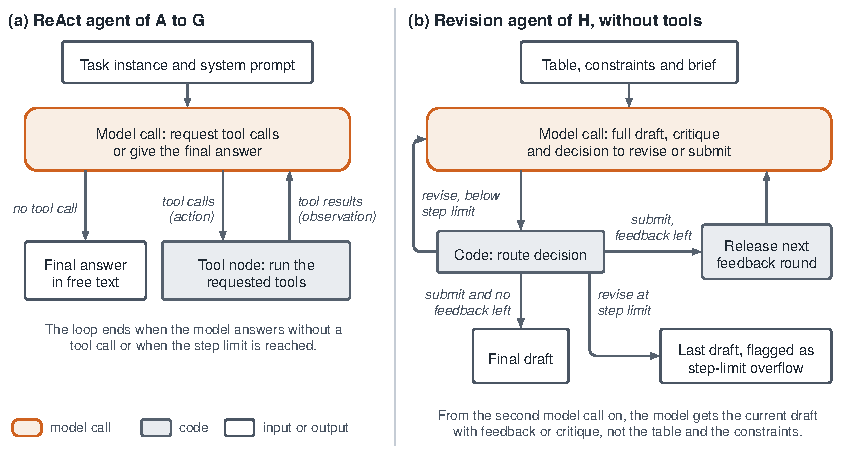
\includegraphics[width=\linewidth]{Figures/fig_agents (1).pdf}
\caption[Control flow of the agents of A to H]{Control flow of the agents of A to H.}
\label{fig:paradigms-agents}
\end{figure}

\begin{figure}[htbp]
\centering
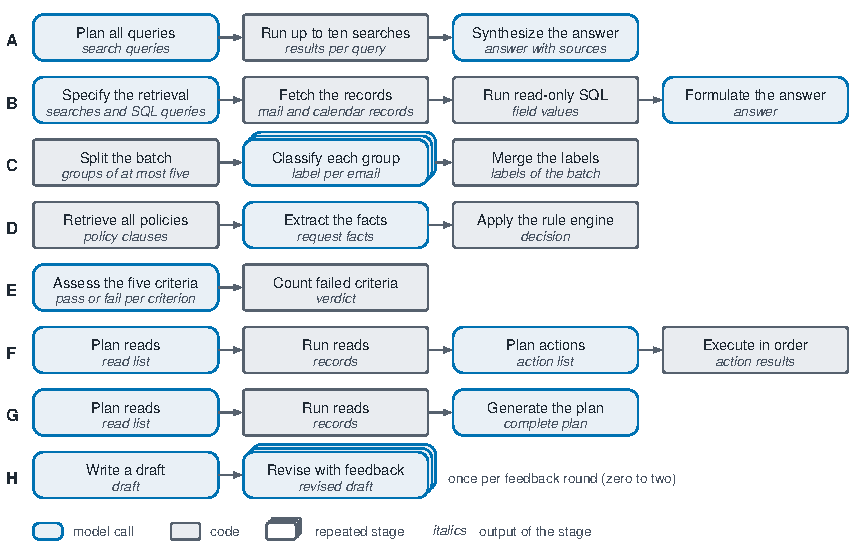
\includegraphics[width=\linewidth]{Figures/fig_workflows.pdf}
\caption[Processing stages of the LLM workflows of A to H]{Processing stages of the LLM workflows of A to H.}
\label{fig:paradigms-workflows}
\end{figure}
\FloatBarrier

The following notes add the implementation details that matter for reading the results.

\paragraph{A. Exploratory research and synthesis.}
\label{app:implementation/a}
The task instances store the reference answer and links to the sources that support it. The LLM workflow groups the search results by query and removes duplicate URLs before the synthesis. Because one model response can request several searches, two agent executions made eleven and fifteen searches despite the recursion limit of 21. The task instances do not rule out that a model knows an answer without searching.

\paragraph{B. Structured data retrieval and transformation.}
\label{app:implementation/b}
The LLM workflow stages the fetched mail and calendar records in temporary tables of its database connection and computes each answer field with read-only SQL; a failing query leaves its field empty. These SQL queries wait for the same synthetic delay as tool calls but are not counted as tool calls. Three agent executions made fifteen, fifteen and seventeen tool calls, so the intended budget of twelve was not a hard cap.

\paragraph{C. Ambiguous classification and disambiguation.}
\label{app:implementation/c}
The group loop runs inside one graph node, so the LLM workflow makes one model call for three or five emails and two for eight. No clean agent execution used the CRM tools.

\paragraph{D. Compliance and rule-based decisioning.}
\label{app:implementation/d}
The LLM workflow retrieves the policy catalogue and every listed document before it extracts the request facts. The rule engine then evaluates the retrieved clauses, so a wrong fact extraction can still lead to a wrong decision. The agent chooses which documents to retrieve.

\paragraph{E. Output verification and quality control.}
\label{app:implementation/e}
The verdict engine maps zero failed criteria to \textit{pass}, one or two to \textit{needs revision} and three or more to \textit{fail}. It stops with an error if the five criteria are not assessed exactly once each, instead of returning a default verdict. No clean agent execution used the CRM tools.

\paragraph{F. Transactional action execution.}
\label{app:implementation/f}
Before each execution, the runner rebuilds the database from the seed records; timing starts afterwards. The backend refuses some case closures under a fixed rule, so a returned refusal can determine the next action. The LLM workflow records failed actions but does not plan again.

\paragraph{G. Strategic and adaptive planning.}
\label{app:implementation/g}
The stored reference plans contain three actions at low, five to seven at medium and fifteen to eighteen at high difficulty; these lengths are not proven optimal. After the execution, a simulator applies the plan to a fresh in-memory copy of the seed records and checks the preconditions of each action and then the goal. A plan with one violated precondition fails as a whole.

\paragraph{H. Content drafting and refinement.}
\label{app:implementation/h}
Because the router checks a submission first, the turn limit in Table~\ref{tab:app-implementations} only stops self-revision. The agent then returns its current draft with an overflow flag.

\subsubsection{Development Decisions}
\label{app:protocol/development}

Task instances and implementations were refined together. The development log records the starting state, decision, result and finding for each iteration. Table~\ref{tab:app-implementation-development} summarizes the decisions needed to understand the retained implementations. The cited IT entries are located in \texttt{docs/iteration\_log.md} in the digital appendix (Appendix~\ref{app:repository}). The table summarizes development evidence; final comparative success rates are reported separately in Section~\ref{subsubsec:TADF/results}.

\begingroup
\renewcommand{\baselinestretch}{1}
\small
\setlength{\tabcolsep}{4pt}
\renewcommand{\arraystretch}{1.08}
\begin{longtable}{>{\raggedright\arraybackslash}p{\dimexpr0.060\linewidth-2\tabcolsep\relax} >{\raggedright\arraybackslash}p{\dimexpr0.280\linewidth-2\tabcolsep\relax} >{\raggedright\arraybackslash}p{\dimexpr0.360\linewidth-2\tabcolsep\relax} >{\raggedright\arraybackslash}p{\dimexpr0.300\linewidth-2\tabcolsep\relax}}
\caption[Development decisions for the implementations]{Development decisions for the implementations.}\label{tab:app-implementation-development} \\
\toprule
\textbf{ID} & \textbf{Starting problem} & \textbf{Development decision} & \textbf{Result and evidence boundary} \\
\midrule
\endfirsthead
\multicolumn{4}{l}{\tablename~\thetable{} (continued)} \\
\toprule
\textbf{ID} & \textbf{Starting problem} & \textbf{Development decision} & \textbf{Result and evidence boundary} \\
\midrule
\endhead
\midrule
\multicolumn{4}{r}{\emph{Continued on the next page.}} \\
\endfoot
\bottomrule
\endlastfoot
A & Familiar facts allowed correct answers without decisive retrieval; compound answers also introduced answer-format effects. & Replace trivia with constructed research questions; distinguish parallel retrieval from linked searches; add checks without tools and single-value endpoints for the high level (IT-031, IT-038, IT-042). & The revised set exercises retrieval dependencies. Checks without tools were used during development, but the stored check lacks model metadata and cannot establish absence of memorization for every model. \\
\addlinespace[2.5pt]
B & Earlier variants mixed retrieval with in-context arithmetic or obscured the intended mail/calendar interfaces. Generated query conventions also caused failures. & Use one retrieval-specification call, tool-based mail/calendar fetching, SQL over CRM and staged records, and one answer call (IT-033, IT-037, IT-043). & The retained implementation separates query construction from deterministic execution. Semantic matching and SQL correctness still depend on the generated specification. \\
\addlinespace[2.5pt]
C & Single-email classification gave little scope for different control behavior. & Construct small email batches and use a fixed chunk size of five in the LLM workflow, retaining the complete batch in the agent context (IT-040, IT-044). & This retains a case where external tools are unnecessary. The tested batches do not establish an advantage for chunking at large context sizes. \\
\addlinespace[2.5pt]
D & With the complete policy inside the prompt, both implementations largely reduced to one model call. & Move policies to a separate registry, add interacting rules and distractors, and separate fact extraction from deterministic policy application (IT-041, IT-045). & The retained contrast concerns applying retrieved rules in code or within the model context. Correct rule execution still requires correctly extracted facts. \\
\addlinespace[2.5pt]
E & The original ranking design was replaced by verdicts; a later version still asked both implementations to apply the complete rubric in one call. & Keep the criterion assessments in one structured model call and move the verdict calculation to code (IT-022, IT-046). & The engine checks criterion coverage and calculates the verdict. The quality of the individual criterion judgments remains model-dependent. \\
\addlinespace[2.5pt]
F & The initial action planner lacked identifiers revealed by reads. Later review found insufficient action-outcome cases and predicates affected by changed seed records. & Add retrieval before action planning; introduce three action-outcome instances; repair predicates and express organizational requirements through runbook excerpts (IT-014, IT-047, IT-049). & Development checks exercised successful actions and prohibited alternatives. The retained LLM workflow can plan from read results but cannot revise its action list during dispatch. The outcome check of f-med-5 was not adjusted to the extended seed and rejects the complete action set (Appendix~\ref{app:results/contrasts}). \\
\addlinespace[2.5pt]
G & Abstract planning tasks did not match the local workplace setting. A later review considered adding further revision or retrieval mechanisms. & Construct CRM scenarios with a plan simulator; retain the two-stage LLM workflow and adaptive retrieval agent, and align the request/runbook wording (IT-023, IT-050, IT-051). & Reference plans and invalid-action cases were tested mechanically. A verifier-driven revision stage was not implemented in the main experimental comparison. \\
\addlinespace[2.5pt]
H & Qualitative ratings alone did not capture violated constraints; early numeric checks rejected valid arithmetic derivations. & Combine deterministic checks with qualitative scoring, permit valid derived numbers, and retain inline data and identical scripted feedback (IT-025--028, IT-052). & Inline data limits retrieval effects. H tests fixed revision stages against model-selected self-revision; judge reliability remains subject to Appendix~\ref{app:protocol/judges}. \\
\end{longtable}
\endgroup

The development checks informed the revisions but did not test the implementations on unused tasks. The main experimental comparison executed the state frozen in IT-053.

\subsubsection{Execution of the Main Experimental Comparison}
\label{app:protocol/execution}

The main experimental comparison ran on 6 and 7 July 2026. It used GPT-5.4-nano, GPT-5.4-mini and GPT-5.2 on the same task instances and implementations; this three-model design replaced the single-model plan of the protocol (D-032, Appendix~\ref{app:protocol/changes}). One batch contains the fifteen task instances of a task archetype, each executed with both orchestration paradigms, which gives thirty executions. The five clean batches per task archetype give forty batches and 1,200 executions. The three models add twenty-four perturbation batches with 252 executions (Appendix~\ref{app:protocol/metrics}).

Table~\ref{tab:app-model-settings} lists the model snapshots, repetitions and reasoning settings. The count in each column applies to one task instance or perturbation variant per orchestration paradigm. All model calls request temperature 0 and seed 42, which did not remove variation between repeated executions. For each model, both orchestration paradigms use the same configuration; the reasoning setting differs between the models.

\begin{table}[htbp]
\centering
\caption[Models and repetitions of the main experimental comparison]{Models and repetitions of the main experimental comparison.}
\label{tab:app-model-settings}
\renewcommand{\baselinestretch}{1}
\small
\setlength{\tabcolsep}{4pt}
\renewcommand{\arraystretch}{1.08}
\begin{tabular}{>{\raggedright\arraybackslash}p{\dimexpr0.380\linewidth-2\tabcolsep\relax} >{\raggedright\arraybackslash}p{\dimexpr0.120\linewidth-2\tabcolsep\relax} >{\raggedright\arraybackslash}p{\dimexpr0.160\linewidth-2\tabcolsep\relax} >{\raggedright\arraybackslash}p{\dimexpr0.340\linewidth-2\tabcolsep\relax}}
\toprule
\textbf{Model snapshot} & \textbf{Clean} & \textbf{Perturbed} & \textbf{Reasoning setting} \\
\midrule
\texttt{gpt-5.4-nano-2026-03-17} & 2 & 1 & Not explicitly set \\
\addlinespace[2.5pt]
\texttt{gpt-5.4-mini-2026-03-17} & 2 & 1 & Not explicitly set \\
\addlinespace[2.5pt]
\texttt{gpt-5.2-2025-12-11} & 1 & 1 & \texttt{reasoning\_effort="none"} \\
\bottomrule
\end{tabular}
\end{table}

The grid runner sets the model and run label for each batch and processes models, runs and task archetypes in a fixed order. The runners of the task archetypes load the task instances, execute both orchestration paradigms, record resource use and apply the outcome checks. The aggregation script combines the result files into one file with 1,452 rows, one per execution, identified by model, run label, task archetype, task instance and orchestration paradigm.

IT-053 records two incidents. A usage limit of the search provider made seven A batches fail: the second GPT-5.4-nano clean batch, both GPT-5.4-mini clean batches, the GPT-5.2 clean batch and the three perturbation batches. Their result files were discarded, and the batches were repeated on 7 July 2026 after a plan upgrade; the first GPT-5.4-nano batch predates the limit and was kept. Provider throttling also lengthened some executions. A request timeout of 300 seconds with three retries was added during the runs, so these client settings were not constant for all batches. The median latency reduces the influence of single long executions but not of the provider conditions.

All other failed executions remain in the data, including recursion-limit failures of the B agent and output-validation failures of the A and F LLM workflows. For GPT-5.4-nano and GPT-5.4-mini, the two clean repetitions give 480 matched combinations of task instance, orchestration paradigm and model, of which 49 changed their task success (10.2 percent). GPT-5.2 ran only one clean repetition, so its repeatability was not measured.

\subsubsection{Design and Execution of the Deep-Dive Runs}
\label{app:protocol/deepdive}

This section documents the deep-dive runs of Section~\ref{subsubsec:TADF/deepdive}. The development log records their planning after the first interpretation of the main experimental comparison (IT-054, IT-055), the construction and execution of the five task families (IT-056 to IT-068) and the confirmation test (IT-069). All task instances were constructed for this study on the local CRM, mail and calendar data. Table~\ref{tab:app-deepdive-design} lists their variants and contrasts.

\begingroup
\renewcommand{\baselinestretch}{1}
\small
\setlength{\tabcolsep}{4pt}
\renewcommand{\arraystretch}{1.08}
\begin{longtable}{>{\raggedright\arraybackslash}p{\dimexpr0.190\linewidth-2\tabcolsep\relax} >{\raggedright\arraybackslash}p{\dimexpr0.170\linewidth-2\tabcolsep\relax} >{\raggedright\arraybackslash}p{\dimexpr0.640\linewidth-2\tabcolsep\relax}}
\caption[Task families and variants of the deep-dive runs]{Task families and variants of the deep-dive runs. Counts refer to task instances, not executions.}\label{tab:app-deepdive-design} \\
\toprule
\textbf{Task family or test} & \textbf{Task instances} & \textbf{Variants and contrasts} \\
\midrule
\endfirsthead
\multicolumn{3}{l}{\tablename~\thetable{} (continued)} \\
\toprule
\textbf{Task family or test} & \textbf{Task instances} & \textbf{Variants and contrasts} \\
\midrule
\endhead
\midrule
\multicolumn{3}{r}{\emph{Continued on the next page.}} \\
\endfoot
\bottomrule
\endlastfoot
P: Plan uncertainty & 20: four variants, five each & P-a: a read determines the number of actions. P-b: the outcomes of earlier actions determine it. P-c: a needed fact lies in the CRM, mail or calendar system, and the task does not name which. P-d: record values determine the order of actions. \\
\addlinespace[2.5pt]
X: Crossed gates & 15: three variants, five each & X-1: written rules applied to the outcomes of closing attempts. X-2: a two-step retrieval chain followed by updates with record-specific values. X-3: written rules, decidable before any action, that require different updates for different records. \\
\addlinespace[2.5pt]
L: Payload scaling & 18: three task shapes, three volumes, two each & L-1: raising the longest-open case. L-2: a uniform bulk update. L-3: finding the oldest email on a topic. The records grow by factors of 1, 5 and 20, from 8 to 160 cases or from 10 to 200 emails, under fixed instruction templates. In the bulk update, the number of actions also grows, from 2 to 40. \\
\addlinespace[2.5pt]
M: State drift & 15: three variants, five each & M-1: a change during the execution that the next tool response reveals. M-2: a change after which an outdated write succeeds without a signal. M-3: as M-2, with an instruction to re-check records before each change. \\
\addlinespace[2.5pt]
S: Staged adaptivity & 15: ten reused, five new & S-1: the five X-1 instances. S-2: the five P-b instances. S-3: five new instances that add a report on the cases closed in the same execution; one of them involves no refusal and serves as a control. \\
\addlinespace[2.5pt]
Confirmation test & Two F instances & Target: reassigning the nine cases of one agent, two of them closed, to another agent (f-med-3). Control: moving seventeen opportunities to another stage (f-med-4). \\
\end{longtable}
\endgroup

\paragraph{Implementations and conditions.}
P, X, L and M reused the LLM workflow and the agent of F without changes (Appendix~\ref{app:implementation/f}). Both orchestration paradigms received the same instruction, including its runbook excerpt. In X, the models applied the written rules themselves; the deterministic rule engine of D was not added. Before each execution, the runner restored the database from the seed data. L then inserted the additional records of the task instance, and M installed its trigger. The trigger closes a second record as soon as the execution first changes a watched record, not after a fixed time. Both orchestration paradigms thus meet the change at the same point of the task, and M does not examine changes before the first write. In M-1, the trigger works in both directions, so the check accepts either order of the two closing operations.

S added a state-machine LLM workflow that keeps the read stage of F. One model call plans each closing step with branches for the three outcomes of the closing tool: closed, refused and already closed. During the execution, code selects the matching branch and inserts only the case identifier and the stated reason into prepared texts. It stops after at most twelve steps and at outcomes without a planned branch. Actions after the last step, such as a final report, receive no inserted values, so their content is fixed when the plan is made. Before the S runs, the log states three hypotheses: the state-machine LLM workflow solves S-1 and S-2 but not S-3, which the agent solves. For the ten reused task instances, only the state-machine LLM workflow was executed; the observations of the LLM workflow and the agent come from X-1 and P-b. The five new task instances were executed with all three implementations.

The map-form LLM workflow of the confirmation test also keeps the read stage of F. A model call lists the items of the task. Code then requests a separate action plan for each item, for at most forty items, and executes it. The comparison uses the GPT-5.2 executions of the original LLM workflow and the agent from the main experimental comparison. Before the test, the log states two hypotheses: the map-form LLM workflow solves the target, and the control remains solved. The log entries IT-049 and IT-069 and the docstrings of the implementation describe the target as nine updates with item-specific owners and notes. The stored task instance and its outcome check, however, require the same new agent for all nine cases. The test therefore examined the complete processing of a list of records with one model call per item, not the binding of different values to different items. IT-083 records this correction and its consequence for the framework (Section~\ref{subsubsec:TADF/evidence}).

\paragraph{Execution and record selection.}
The standard runs of the five task families used the models and settings of the main experimental comparison (Appendix~\ref{app:protocol/execution}) in five model/run configurations: two repetitions each for GPT-5.4-nano and GPT-5.4-mini and one for GPT-5.2. They took place from 16 to 22 July 2026 and contain 805 new executions: 200 for P, 150 for X, 180 for L, 150 for M and 125 for S. S also reuses 100 observations from X-1 and P-b, which are not new executions. Because GPT-5.2 had only one repetition, a supplementary GPT-5.2 repetition of P-c added ten executions on 22 July 2026. The confirmation test on 3 August 2026 comprises two GPT-5.2 executions on each of its two task instances and one preliminary GPT-5.4-nano execution on the target. Preliminary runs of the families are stored separately and excluded from the comparisons. The result files under \path{data/results/phase2b/} record the model, run label, task family, task instance and implementation. After a re-execution, the analysis keeps the latest observation for each combination of these identifiers. Executions that ended with an exception count as unsuccessful and have no token record; this applies to 26 of the 805.

\paragraph{Checks and corrections.}
Each construction script tests every outcome check twice: it must fail on the unchanged initial state and pass after the specified correct actions. Before the standard runs, one outcome check of P and the instructions of the state-machine LLM workflow were adjusted (IT-056, IT-067). During the runs, the expected result of one P-d instance, the mail search and the closing tool were corrected for both orchestration paradigms (IT-057, IT-062, IT-064). The affected P-d instance, the six L email instances and the five M-1 instances were executed again. All runs of P and X, including the repeated P-d instance, preceded the two tool corrections and were not repeated after them; of P-c, only the supplementary GPT-5.2 repetition ran afterwards.

The repository contains the construction scripts and runners, both additional LLM workflows, the analysis notebook of the deep-dive runs and the development log (Appendix~\ref{app:repository}).

\subsubsection{Protocol and Implemented Procedure}
\label{app:protocol/changes}

The experimental protocol was written before the task archetypes were implemented (IT-001, IT-002). It specified the compared conditions, the task corpus, the tool infrastructure, the execution procedure, the metrics and the statistical analysis. It was not registered publicly. Deviations during development were recorded as D-001 to D-032. The protocol lists 20 of them; the other twelve appear only in the development log. Several deviations were also written into the protocol text, for example the local database (D-001), the hash-based delays (D-005) and the deterministic checks of E and G (D-011, D-012). Table~\ref{tab:app-protocol-changes} lists where the implemented procedure still differs from the protocol or from later plans in the development log. Where plans and records differ, the code and result files describe what was executed. The repository contains the protocol in its last version (Appendix~\ref{app:repository}).

\begingroup
\renewcommand{\baselinestretch}{1}
\small
\setlength{\tabcolsep}{4pt}
\renewcommand{\arraystretch}{1.08}
\begin{longtable}{>{\raggedright\arraybackslash}p{\dimexpr0.170\linewidth-2\tabcolsep\relax} >{\raggedright\arraybackslash}p{\dimexpr0.320\linewidth-2\tabcolsep\relax} >{\raggedright\arraybackslash}p{\dimexpr0.380\linewidth-2\tabcolsep\relax} >{\raggedright\arraybackslash}p{\dimexpr0.130\linewidth-2\tabcolsep\relax}}
\caption[Differences between the planned and the implemented procedure]{Differences between the planned and the implemented procedure. \emph{Planned} refers to the protocol or, where named, to a later plan in the development log. \emph{Record} names the deviation (D) or log entry (IT); a dash marks a difference that was identified only when this thesis was written.}\label{tab:app-protocol-changes} \\
\toprule
\textbf{Aspect} & \textbf{Planned} & \textbf{Implemented} & \textbf{Record} \\
\midrule
\endfirsthead
\multicolumn{4}{l}{\tablename~\thetable{} (continued)} \\
\toprule
\textbf{Aspect} & \textbf{Planned} & \textbf{Implemented} & \textbf{Record} \\
\midrule
\endhead
\midrule
\multicolumn{4}{r}{\emph{Continued on the next page.}} \\
\endfoot
\bottomrule
\endlastfoot
Conditions & Always LLM workflow, Always agent, a difficulty-only router and a TADF router; the routers select between recorded executions. & Only the two orchestration paradigms were executed; no difficulty-only router was built. Routing was examined retrospectively (Section~\ref{subsubsec:TADF/functionality}) and on WorkBench (Section~\ref{subsubsec:TADF/episode2}). & -- \\
\addlinespace[2.5pt]
Models and repetitions & One model, GPT-5.2; one execution per task instance and orchestration paradigm; 240 plus 48 perturbation executions. & Three models; two clean repetitions each for GPT-5.4-nano and GPT-5.4-mini, one for GPT-5.2; 1,200 clean plus 252 perturbation executions. & D-032 \\
\addlinespace[2.5pt]
Task instances & Taken from benchmark sources with their original meaning; own construction only where no source fits. & All 120 constructed for this study; benchmark sources supplied task patterns (Appendix~\ref{app:taxonomy/sources}). & e.g.\ D-012, D-016 \\
\addlinespace[2.5pt]
Reasoning setting & \texttt{reasoning\_effort} set to \texttt{"none"} for all executions. & Set only for GPT-5.2; provider default for the GPT-5.4 models. & IT-053 \\
\addlinespace[2.5pt]
Step limits & One per task archetype, e.g.\ 2/6/10 steps in F and 5/12/25 in G; exceeding it counts as failure. & For the agents of A, B, C, G and H; no task-specific limit for the agents of D, E and F. & D-007, D-012 \\
\addlinespace[2.5pt]
Workflow nodes & At most one model call per graph node. & In C, one node classifies all groups of a batch, with two model calls for eight emails. & IT-044 \\
\addlinespace[2.5pt]
Database reset & Seed state restored before each execution. & Restored before each F execution only. F alone changes the database; the other task archetypes read the state left by the preceding F execution. & -- \\
\addlinespace[2.5pt]
Success in A & Quality score from a rubric-based judgment against the expected answer. & Binary judge decision whether the answer states the reference fact. & IT-008 \\
\addlinespace[2.5pt]
Success in H & Judge quality score as primary measure; deterministic checks reported alongside (D-013). & Solved if all deterministic checks pass; judge quality score complementary. & -- \\
\addlinespace[2.5pt]
Judge agreement & Weighted $\kappa\geq0.6$ on a human-rated 20 percent sample; if missed, judge ratings discarded and a second human reviewer rates. & A: $\kappa=1.000$. H: $\kappa=0.348$; judge score kept as complementary measure, AC1 reported, no second reviewer. & D-015 \\
\addlinespace[2.5pt]
Judge model & Fixed GPT-5.2 judge for all models (IT-053). & Model of the judged execution; no separate judge model recorded. & -- \\
\addlinespace[2.5pt]
Error rate & Share of executions ending with incorrect output or iteration overflow. & Share with a recorded error or iteration overflow; incorrect output counts only as failed task success. & -- \\
\addlinespace[2.5pt]
Robustness & Relative drop in success on a 20 percent subset with synonyms and irrelevant sentences; IT-053: only base tasks solved in all clean executions of a model. & Success rate on 42 fixed variants (35 percent of the task instances) with varied wording changes, without this restriction. & -- \\
\addlinespace[2.5pt]
Analysis & Per task archetype and difficulty level: paired Wilcoxon tests, Cliff's delta with bootstrap intervals and Holm correction; an equally weighted aggregate score; an efficiency frontier. & Descriptive rates and resource summaries. The planned tests, effect sizes and efficiency frontier were computed afterwards, when this thesis was written (\path{statistical_analysis.ipynb}). No combination reaches $p<0.05$; for five pairs, the exact two-sided Wilcoxon $p$-value is at least 0.0625. The aggregate score was not computed, because the protocol left its normalization open. & -- \\
\addlinespace[2.5pt]
Deep-dive runs & Not planned. & Five task families and a confirmation test after the main experimental comparison for questions it left open (Section~\ref{subsubsec:TADF/deepdive}). & IT-054 to IT-069 \\
\end{longtable}
\endgroup

% Appendix D: Detailed Experimental Results

\subsection{Detailed Experimental Results}
\label{app:results}

This appendix contains the detailed tables for Section~\ref{subsubsec:TADF/results}. D.1 and D.2 cover the main experimental comparison, and D.3 and D.4 the deep-dive runs. The notebook \path{statistical_analysis.ipynb} reproduces each table of Section~\ref{subsubsec:TADF/results} and of this appendix from the stored result files and prints it under its label (Appendix~\ref{app:repository}). Counts give successful executions over all executions of the stated group. Token values use the executions with a token record; missing records are not treated as zero. W denotes the LLM workflow, and the letters A--H denote the task archetypes as in Table~\ref{tab:grid-results}.

\subsubsection{Main Experimental Comparison}
\label{app:results/main}

Table~\ref{tab:app-intervals} reports the differences between the orchestration paradigms with their uncertainty. The intervals are 95 percent percentile bootstrap intervals over task instances with 10,000 resamples, so the repeated executions of a task instance stay together. The exact sign-flip test compares the mean difference over the 15 task instances with all sign assignments, and Holm's correction covers the eight task archetypes. The notebook also gives the intervals for each model.

\begin{table}[htbp]
\centering
\caption[Success differences and token ratios with 95 percent intervals]{Success differences and token ratios with 95 percent intervals.}
\label{tab:app-intervals}
\renewcommand{\baselinestretch}{1}
\footnotesize
\setlength{\tabcolsep}{3pt}
\renewcommand{\arraystretch}{1.08}
\begin{tabular*}{\linewidth}{@{\extracolsep{\fill}}l c c c c@{}}
\toprule
\textbf{ID} & \textbf{Success, W $-$ Agent (pp)} & \textbf{Sign-flip $p$} & \textbf{Holm $p$} & \textbf{Token cost, Agent/W} \\
\midrule
A & $-$10.7 [$-$25.3, 4.0] & 0.254 & 1.000 & 2.03 [1.26, 2.86] \\
B & $-$12.0 [$-$32.0, 5.3] & 0.313 & 1.000 & 7.91 [4.17, 12.49] \\
C & $-$2.7 [$-$8.0, 0.0] & 1.000 & 1.000 & 0.85 [0.76, 0.95] \\
D & 20.0 [9.3, 32.0] & 0.008 & 0.063 & 6.16 [6.15, 6.17] \\
E & 8.0 [$-$6.7, 21.4] & 0.391 & 1.000 & 0.90 [0.89, 0.90] \\
F & $-$26.7 [$-$48.0, $-$8.0] & 0.047 & 0.281 & 4.34 [2.78, 6.40] \\
G & $-$13.3 [$-$36.0, 8.0] & 0.324 & 1.000 & 2.89 [2.28, 3.59] \\
H & 14.7 [5.3, 26.7] & 0.031 & 0.219 & 1.49 [1.32, 1.72] \\
\bottomrule
\end{tabular*}
\par\smallskip
\begin{minipage}{\linewidth}\footnotesize
pp: percentage points; brackets: 95 percent intervals. Token cost, Agent/W: the agent's mean token cost divided by the LLM workflow's.
\end{minipage}
\end{table}

Table~\ref{tab:app-token-results} relates token cost to success. Tokens per success divide the recorded tokens of all executions, including unsuccessful ones, by the number of successful executions. Executions without a token record add no tokens, so the values of the LLM workflow in A and F and of the agent in B are slightly too low. The median of the eight ratios is 2.21.

\begin{table}[htbp]
\centering
\caption[Token cost per successful execution]{Token cost per successful execution.}
\label{tab:app-token-results}
\renewcommand{\baselinestretch}{1}
\footnotesize
\setlength{\tabcolsep}{3pt}
\renewcommand{\arraystretch}{1.08}
\begin{tabular}{>{\raggedright\arraybackslash}p{\dimexpr0.12\linewidth-2\tabcolsep\relax} *{8}{>{\raggedleft\arraybackslash}p{\dimexpr0.11\linewidth-2\tabcolsep\relax}}}
\toprule
 & \textbf{A} & \textbf{B} & \textbf{C} & \textbf{D} & \textbf{E} & \textbf{F} & \textbf{G} & \textbf{H} \\
\midrule
W & 7,547 & 3,197 & 1,713 & 903 & 1,725 & 8,389 & 5,891 & 3,214 \\
Agent & 13,555 & 20,515 & 1,415 & 6,953 & 1,722 & 23,471 & 13,996 & 6,592 \\
Agent/W & 1.80 & 6.42 & 0.83 & 7.70 & 1.00 & 2.80 & 2.38 & 2.05 \\
\bottomrule
\end{tabular}
\end{table}

Table~\ref{tab:app-robustness-results} reports task success on the perturbation variants: fifteen executions per orchestration paradigm, eighteen in D and G. Because not all base task instances were solved in every clean execution, these rates combine baseline difficulty with sensitivity to the changed wording (Appendix~\ref{app:protocol/metrics}).

\begin{table}[htbp]
\centering
\caption[Task success on the perturbation variants]{Task success on the perturbation variants.}
\label{tab:app-robustness-results}
\renewcommand{\baselinestretch}{1}
\footnotesize
\setlength{\tabcolsep}{3pt}
\renewcommand{\arraystretch}{1.08}
\begin{tabular}{>{\raggedright\arraybackslash}p{\dimexpr0.12\linewidth-2\tabcolsep\relax} *{8}{>{\raggedleft\arraybackslash}p{\dimexpr0.11\linewidth-2\tabcolsep\relax}}}
\toprule
 & \textbf{A} & \textbf{B} & \textbf{C} & \textbf{D} & \textbf{E} & \textbf{F} & \textbf{G} & \textbf{H} \\
\midrule
W & 12/15 & 13/15 & 15/15 & 18/18 & 15/15 & 13/15 & 17/18 & 13/15 \\
Agent & 13/15 & 15/15 & 15/15 & 13/18 & 14/15 & 15/15 & 16/18 & 13/15 \\
\bottomrule
\end{tabular}
\end{table}

Most failures carried no error signal. Seven of the 1,200 executions ended with a recorded error or step-limit overflow; all others returned a result, which the outcome check accepted or rejected. In D, the LLM workflow returned the reference decision in all 75 executions. Twelve of the agent's fifteen incorrect decisions were less restrictive than the reference: seven escalations instead of a decline, four approvals instead of an escalation and one lower escalation level. In E, the criterion assessments of the LLM workflow in its 90 scored clean and perturbation executions contained 35 false fails, which mark a satisfied criterion as failed, and 17 missed fails, which overlook a failed criterion.
\FloatBarrier

\subsubsection{Difficulty Levels and Task Requirements}
\label{app:results/contrasts}

Table~\ref{tab:app-difficulty-results} reports task success by difficulty level. The levels are defined per task archetype (Table~\ref{tab:app-difficulty}) and form no common scale. Table~\ref{tab:app-high-model-results} separates the high level by model.

\begin{table}[htbp]
\centering
\caption[Task success by difficulty level]{Task success by difficulty level.}
\label{tab:app-difficulty-results}
\renewcommand{\baselinestretch}{1}
\footnotesize
\setlength{\tabcolsep}{3pt}
\renewcommand{\arraystretch}{1.08}
\begin{tabular}{>{\raggedright\arraybackslash}p{\dimexpr0.064\linewidth-2\tabcolsep\relax} >{\raggedright\arraybackslash}p{\dimexpr0.306\linewidth-2\tabcolsep\relax} *{6}{>{\centering\arraybackslash}p{\dimexpr0.105\linewidth-2\tabcolsep\relax}}}
\toprule
 & & \multicolumn{2}{c}{\textbf{Low}} & \multicolumn{2}{c}{\textbf{Medium}} & \multicolumn{2}{c}{\textbf{High}} \\
\cmidrule(lr){3-4}\cmidrule(lr){5-6}\cmidrule(lr){7-8}
\textbf{ID} & \textbf{Varied demand} & \textbf{W} & \textbf{Agent} & \textbf{W} & \textbf{Agent} & \textbf{W} & \textbf{Agent} \\
\midrule
A & Sources, search chain & 21/25 & 19/25 & 19/25 & 20/25 & 14/25 & 23/25 \\
B & Systems combined & 25/25 & 25/25 & 16/25 & 23/25 & 8/25 & 10/25 \\
C & Ambiguity, batch size & 25/25 & 25/25 & 23/25 & 25/25 & 25/25 & 25/25 \\
D & Rule interaction & 25/25 & 22/25 & 25/25 & 18/25 & 25/25 & 20/25 \\
E & Subtlety of failures & 21/25 & 20/25 & 19/25 & 17/25 & 19/25 & 16/25 \\
F & Action scope, dependence & 20/25 & 20/25 & 13/25 & 20/25 & 2/25 & 15/25 \\
G & Plan length & 16/25 & 22/25 & 19/25 & 20/25 & 11/25 & 14/25 \\
H & Constraints, feedback & 21/25 & 20/25 & 18/25 & 9/25 & 1/25 & 0/25 \\
\bottomrule
\end{tabular}
\end{table}

\begin{table}[htbp]
\centering
\caption[Task success at the high difficulty level by model]{Task success at the high difficulty level by model.}
\label{tab:app-high-model-results}
\renewcommand{\baselinestretch}{1}
\footnotesize
\setlength{\tabcolsep}{3pt}
\renewcommand{\arraystretch}{1.08}
\begin{tabular}{>{\raggedright\arraybackslash}p{\dimexpr0.064\linewidth-2\tabcolsep\relax} *{6}{>{\centering\arraybackslash}p{\dimexpr0.156\linewidth-2\tabcolsep\relax}}}
\toprule
 & \multicolumn{2}{c}{\textbf{GPT-5.4-nano}} & \multicolumn{2}{c}{\textbf{GPT-5.4-mini}} & \multicolumn{2}{c}{\textbf{GPT-5.2}} \\
\cmidrule(lr){2-3}\cmidrule(lr){4-5}\cmidrule(lr){6-7}
\textbf{ID} & \textbf{W} & \textbf{Agent} & \textbf{W} & \textbf{Agent} & \textbf{W} & \textbf{Agent} \\
\midrule
A & 3/10 & 9/10 & 7/10 & 9/10 & 4/5 & 5/5 \\
B & 3/10 & 5/10 & 5/10 & 2/10 & 0/5 & 3/5 \\
C & 10/10 & 10/10 & 10/10 & 10/10 & 5/5 & 5/5 \\
D & 10/10 & 8/10 & 10/10 & 8/10 & 5/5 & 4/5 \\
E & 5/10 & 7/10 & 9/10 & 5/10 & 5/5 & 4/5 \\
F & 1/10 & 4/10 & 0/10 & 7/10 & 1/5 & 4/5 \\
G & 2/10 & 3/10 & 6/10 & 7/10 & 3/5 & 4/5 \\
H & 0/10 & 0/10 & 0/10 & 0/10 & 1/5 & 0/5 \\
\bottomrule
\end{tabular}
\end{table}

Table~\ref{tab:app-main-contrasts} lists the fifteen task instances of F. In f-high-1, f-high-2 and f-high-5, a later action depends on the outcome of an earlier one. In f-low-2, the closing tool refuses the case with the message that an automatic close is not permitted, while the outcome check expects the status `Closed'. All its executions stopped after the refusal, and the agents reported it.

\begin{table}[htbp]
\centering
\caption[Task success in action execution (F) by task instance]{Task success in action execution (F) by task instance.}
\label{tab:app-main-contrasts}
\renewcommand{\baselinestretch}{1}
\footnotesize
\setlength{\tabcolsep}{4pt}
\renewcommand{\arraystretch}{1.08}
\begin{tabular}{>{\raggedright\arraybackslash}p{\dimexpr0.13\linewidth-2\tabcolsep\relax} >{\raggedright\arraybackslash}p{\dimexpr0.67\linewidth-2\tabcolsep\relax} >{\centering\arraybackslash}p{\dimexpr0.1\linewidth-2\tabcolsep\relax} >{\centering\arraybackslash}p{\dimexpr0.1\linewidth-2\tabcolsep\relax}}
\toprule
\textbf{Instance} & \textbf{Required actions} & \textbf{W} & \textbf{Agent} \\
\midrule
f-low-1 & Send one email with given recipient, subject and body & 5/5 & 5/5 \\
f-low-2 & Set one case to `Closed'; the closing tool refuses it & 0/5 & 0/5 \\
f-low-3 & Create one calendar event with all details given & 5/5 & 5/5 \\
f-low-4 & Delete one email by its identifier & 5/5 & 5/5 \\
f-low-5 & Change the priority of one case & 5/5 & 5/5 \\
f-med-1 & Set the four open cases of one agent to `In Progress' & 5/5 & 5/5 \\
f-med-2 & Book one call; a calendar read decides the time slot & 1/5 & 5/5 \\
f-med-3 & Reassign the nine cases of one agent, two of them closed & 2/5 & 5/5 \\
f-med-4 & Move seventeen opportunities to another stage & 5/5 & 5/5 \\
f-med-5\textsuperscript{a} & Email the primary contact of every account in one region & 0/5 & 0/5 \\
f-high-1 & Close two cases; each closing outcome selects its email & 0/5 & 3/5 \\
f-high-2 & Close a duplicate case; if refused, change nothing and escalate & 0/5 & 5/5 \\
f-high-3 & Invite the primary contacts of accounts with won opportunities in a region & 2/5 & 1/5 \\
f-high-4 & Email the agent with the most open cases in one team & 0/5 & 1/5 \\
f-high-5 & Close a case; the customer email depends on the outcome & 0/5 & 5/5 \\
\midrule
\multicolumn{2}{l}{Outcome-dependent task instances: f-high-1, f-high-2, f-high-5} & 0/15 & 13/15 \\
\multicolumn{2}{l}{Other twelve task instances} & 35/60 & 42/60 \\
\bottomrule
\end{tabular}
\par\smallskip
\begin{minipage}{\linewidth}\footnotesize
\textsuperscript{a}\,The outcome check cannot be met with the seed used in the runs; see the text.
\end{minipage}
\end{table}

The outcome check of f-med-5 cannot be met. It lists the primary contacts of seven accounts in the named region and rejects emails to any other recipient. Before the main experimental comparison, the named-customer data of B's retrieval tasks added an eighth account in this region to the shared seed (IT-035). IT-047 later repaired other checks affected by this extension, but not this one. An execution that emails all eight primary contacts therefore counts as a failure; the notebook reproduces this with the stored seed. All five agent executions and two LLM-workflow executions sent eight emails; the result files do not record the recipients. The results of f-med-5 therefore do not measure task success. Without f-med-5, F's counts are 35/70 for the LLM workflow and 55/70 for the agent. The sign-flip test is unchanged, because both orchestration paradigms failed all executions of f-med-5. The same extension added a seventeenth opportunity in the stage of f-med-4, whose check derives its targets from the seed. It also added two accounts with won opportunities in the region of f-high-3. This check requires the six original accounts and accepts events for further accounts, so it accepts complete executions but would also accept executions that omit the two added accounts.
\FloatBarrier

\subsubsection{Deep-Dive Task Families}
\label{app:results/deepdive}

The deep-dive runs used five standard model/run configurations: two repetitions each with GPT-5.4-nano and GPT-5.4-mini and one with GPT-5.2 (Appendix~\ref{app:protocol/deepdive}). Table~\ref{tab:app-deep-model-results} separates them by model. Each variant in P, X, M and S has five task instances, each task shape in L six.

\begin{table}[htbp]
\centering
\caption[Task success in the deep-dive runs by model]{Task success in the deep-dive runs by model.}
\label{tab:app-deep-model-results}
\renewcommand{\baselinestretch}{1}
\footnotesize
\setlength{\tabcolsep}{3pt}
\renewcommand{\arraystretch}{1.08}
\begin{tabular}{>{\raggedright\arraybackslash}p{\dimexpr0.11\linewidth-2\tabcolsep\relax} *{9}{>{\centering\arraybackslash}p{\dimexpr0.0988\linewidth-2\tabcolsep\relax}}}
\toprule
 & \multicolumn{3}{c}{\textbf{GPT-5.4-nano}} & \multicolumn{3}{c}{\textbf{GPT-5.4-mini}} & \multicolumn{3}{c}{\textbf{GPT-5.2}} \\
\cmidrule(lr){2-4}\cmidrule(lr){5-7}\cmidrule(lr){8-10}
\textbf{Variant} & \textbf{W} & \textbf{Agent} & \textbf{SM} & \textbf{W} & \textbf{Agent} & \textbf{SM} & \textbf{W} & \textbf{Agent} & \textbf{SM} \\
\midrule
P-a & 10/10 & 10/10 & -- & 10/10 & 10/10 & -- & 5/5 & 5/5 & -- \\
P-b & 0/10 & 7/10 & -- & 0/10 & 3/10 & -- & 0/5 & 5/5 & -- \\
P-c & 3/10 & 10/10 & -- & 6/10 & 10/10 & -- & 3/5 & 4/5 & -- \\
P-d & 3/10 & 5/10 & -- & 6/10 & 7/10 & -- & 5/5 & 5/5 & -- \\
X-1 & 0/10 & 9/10 & -- & 0/10 & 10/10 & -- & 0/5 & 5/5 & -- \\
X-2 & 0/10 & 10/10 & -- & 0/10 & 9/10 & -- & 0/5 & 5/5 & -- \\
X-3 & 1/10 & 4/10 & -- & 4/10 & 10/10 & -- & 5/5 & 5/5 & -- \\
L-1 & 11/12 & 12/12 & -- & 12/12 & 12/12 & -- & 6/6 & 6/6 & -- \\
L-2 & 11/12 & 12/12 & -- & 12/12 & 12/12 & -- & 6/6 & 6/6 & -- \\
L-3 & 11/12 & 12/12 & -- & 11/12 & 12/12 & -- & 6/6 & 6/6 & -- \\
M-1 & 0/10 & 10/10 & -- & 0/10 & 10/10 & -- & 0/5 & 5/5 & -- \\
M-2 & 0/10 & 0/10 & -- & 0/10 & 0/10 & -- & 0/5 & 0/5 & -- \\
M-3 & 0/10 & 5/10 & -- & 0/10 & 6/10 & -- & 0/5 & 5/5 & -- \\
S-1 & 0/10 & 9/10 & 9/10 & 0/10 & 10/10 & 5/10 & 0/5 & 5/5 & 5/5 \\
S-2 & 0/10 & 7/10 & 4/10 & 0/10 & 3/10 & 5/10 & 0/5 & 5/5 & 5/5 \\
S-3 & 0/10 & 5/10 & 1/10 & 1/10 & 4/10 & 1/10 & 1/5 & 4/5 & 2/5 \\
\bottomrule
\end{tabular}
\par\smallskip
\begin{minipage}{\linewidth}\footnotesize
W: original LLM workflow; SM: state-machine LLM workflow; a dash marks an implementation that was not executed. Table~\ref{tab:deepdive-results} describes the variants.
\end{minipage}
\end{table}

Table~\ref{tab:app-family-results} reports the mean token cost. Token records are missing for 26 of the 805 standard executions, which ended with an exception and count as unsuccessful. Superscripts give the number of records where it is smaller than the number of executions. The ratios compare recorded means. In S-1, six unsuccessful executions of the state-machine LLM workflow have no record, so its mean rests on nineteen executions.

\begin{table}[htbp]
\centering
\caption[Token cost in the deep-dive runs]{Token cost in the deep-dive runs.}
\label{tab:app-family-results}
\renewcommand{\baselinestretch}{1}
\footnotesize
\setlength{\tabcolsep}{4pt}
\renewcommand{\arraystretch}{1.08}
\begin{tabular}{>{\raggedright\arraybackslash}p{\dimexpr0.12\linewidth-2\tabcolsep\relax} *{3}{>{\raggedleft\arraybackslash}p{\dimexpr0.18\linewidth-2\tabcolsep\relax}} *{2}{>{\centering\arraybackslash}p{\dimexpr0.17\linewidth-2\tabcolsep\relax}}}
\toprule
 & \multicolumn{3}{c}{\textbf{Mean token cost}} & \multicolumn{2}{c}{\textbf{Ratio}} \\
\cmidrule(lr){2-4}\cmidrule(lr){5-6}
\textbf{Variant} & \textbf{W} & \textbf{Agent} & \textbf{SM} & \textbf{Agent/W} & \textbf{SM/Agent} \\
\midrule
P-a & 3,346 & 9,393 & -- & 2.81 & -- \\
P-b & 4,084\textsuperscript{[24]} & 19,099 & -- & 4.68 & -- \\
P-c & 4,534\textsuperscript{[24]} & 13,335 & -- & 2.94 & -- \\
P-d & 4,177 & 29,723 & -- & 7.12 & -- \\
X-1 & 4,074\textsuperscript{[20]} & 14,356 & -- & 3.52 & -- \\
X-2 & 3,664\textsuperscript{[24]} & 13,790 & -- & 3.76 & -- \\
X-3 & 3,768 & 11,122 & -- & 2.95 & -- \\
L-1 & 4,924 & 16,461 & -- & 3.34 & -- \\
L-2 & 5,414 & 12,555 & -- & 2.32 & -- \\
L-3 & 9,857 & 22,504 & -- & 2.28 & -- \\
M-1 & 3,754\textsuperscript{[17]} & 14,042 & -- & 3.74 & -- \\
M-2 & 3,390\textsuperscript{[24]} & 20,647 & -- & 6.09 & -- \\
M-3 & 3,522 & 13,140 & -- & 3.73 & -- \\
S-1 & 4,074\textsuperscript{[20]} & 14,356 & 5,004\textsuperscript{[19]} & 3.52 & 0.35 \\
S-2 & 4,084\textsuperscript{[24]} & 19,099 & 5,202 & 4.68 & 0.27 \\
S-3 & 4,363\textsuperscript{[23]} & 18,204\textsuperscript{[24]} & 5,255 & 4.17 & 0.29 \\
\bottomrule
\end{tabular}
\end{table}

Table~\ref{tab:app-payload-results} separates L by record volume. Token cost rose with volume in each task shape for both orchestration paradigms. The agent's cost rose by more tokens in all three task shapes, but by a larger factor only in L-1. In L-2, the number of actions also grows with volume. Token counts accumulate over the model calls of an execution, so they do not measure the largest context of a single call.

\begin{table}[htbp]
\centering
\caption[Payload scaling in L by record volume]{Payload scaling in L by record volume.}
\label{tab:app-payload-results}
\renewcommand{\baselinestretch}{1}
\footnotesize
\setlength{\tabcolsep}{4pt}
\renewcommand{\arraystretch}{1.08}
\begin{tabular}{>{\raggedright\arraybackslash}p{\dimexpr0.16\linewidth-2\tabcolsep\relax} >{\centering\arraybackslash}p{\dimexpr0.12\linewidth-2\tabcolsep\relax} *{2}{>{\centering\arraybackslash}p{\dimexpr0.16\linewidth-2\tabcolsep\relax}} *{2}{>{\raggedleft\arraybackslash}p{\dimexpr0.2\linewidth-2\tabcolsep\relax}}}
\toprule
 & & \multicolumn{2}{c}{\textbf{Task success}} & \multicolumn{2}{c}{\textbf{Mean token cost}} \\
\cmidrule(lr){3-4}\cmidrule(lr){5-6}
\textbf{Task shape} & \textbf{Volume} & \textbf{W} & \textbf{Agent} & \textbf{W} & \textbf{Agent} \\
\midrule
L-1 & $\times$1 & 10/10 & 10/10 & 3,259 & 9,366 \\
L-1 & $\times$5 & 10/10 & 10/10 & 4,153 & 12,737 \\
L-1 & $\times$20 & 9/10 & 10/10 & 7,360 & 27,281 \\
\addlinespace[2.5pt]
L-2 & $\times$1 & 10/10 & 10/10 & 3,173 & 8,822 \\
L-2 & $\times$5 & 10/10 & 10/10 & 4,224 & 11,166 \\
L-2 & $\times$20 & 9/10 & 10/10 & 8,844 & 17,678 \\
\addlinespace[2.5pt]
L-3 & $\times$1 & 9/10 & 10/10 & 3,730 & 10,219 \\
L-3 & $\times$5 & 9/10 & 10/10 & 7,066 & 16,705 \\
L-3 & $\times$20 & 10/10 & 10/10 & 18,774 & 40,590 \\
\bottomrule
\end{tabular}
\par\smallskip
\begin{minipage}{\linewidth}\footnotesize
Two task instances per row, executed in the five standard configurations. L-1: raise the longest-open case; L-2: uniform bulk update; L-3: find the oldest email on a topic.
\end{minipage}
\end{table}
\FloatBarrier

\subsubsection{Supplementary Observations and Confirmation Test}
\label{app:results/supplementary}

Table~\ref{tab:app-p-recheck} compares the standard GPT-5.2 repetition of P-c with the supplementary one. Across both repetitions, the LLM workflow solved 5 of 10 executions and the agent 9 of 10. The standard repetition ran before the correction of the mail search, the supplementary one after it (Appendix~\ref{app:protocol/deepdive}). The supplementary executions are not part of the standard counts and token means.

\begin{table}[htbp]
\centering
\caption[Supplementary GPT-5.2 repetition of P-c]{Supplementary GPT-5.2 repetition of P-c.}
\label{tab:app-p-recheck}
\renewcommand{\baselinestretch}{1}
\footnotesize
\setlength{\tabcolsep}{4pt}
\renewcommand{\arraystretch}{1.08}
\begin{tabular}{>{\raggedright\arraybackslash}p{\dimexpr0.28\linewidth-2\tabcolsep\relax} *{2}{>{\centering\arraybackslash}p{\dimexpr0.17\linewidth-2\tabcolsep\relax}} *{2}{>{\raggedleft\arraybackslash}p{\dimexpr0.19\linewidth-2\tabcolsep\relax}}}
\toprule
 & \multicolumn{2}{c}{\textbf{Task success}} & \multicolumn{2}{c}{\textbf{Mean token cost}} \\
\cmidrule(lr){2-3}\cmidrule(lr){4-5}
\textbf{Repetition} & \textbf{W} & \textbf{Agent} & \textbf{W} & \textbf{Agent} \\
\midrule
Standard (run 1) & 3/5 & 4/5 & 5,892 & 14,279 \\
Supplementary (run 2) & 2/5 & 5/5 & 6,077 & 11,502 \\
\bottomrule
\end{tabular}
\end{table}

Table~\ref{tab:app-map-confirmation} reports the confirmation test by task instance, model and implementation. The original LLM workflow and the agent contribute their single GPT-5.2 execution of each task instance from the main experimental comparison, the map-form LLM workflow two executions. The unsuccessful GPT-5.2 target execution of the map-form LLM workflow processed six of the nine cases. On both task instances, the map-form LLM workflow used more tokens than the original agent. The preliminary GPT-5.4-nano execution is shown separately and is not part of the comparison.

\begin{table}[htbp]
\centering
\caption[Confirmation test of the map-form LLM workflow]{Confirmation test of the map-form LLM workflow.}
\label{tab:app-map-confirmation}
\renewcommand{\baselinestretch}{1}
\footnotesize
\setlength{\tabcolsep}{3pt}
\renewcommand{\arraystretch}{1.08}
\begin{tabular}{>{\raggedright\arraybackslash}p{\dimexpr0.34\linewidth-2\tabcolsep\relax} *{3}{>{\centering\arraybackslash}p{\dimexpr0.095\linewidth-2\tabcolsep\relax}} *{3}{>{\raggedleft\arraybackslash}p{\dimexpr0.125\linewidth-2\tabcolsep\relax}}}
\toprule
 & \multicolumn{3}{c}{\textbf{Task success}} & \multicolumn{3}{c}{\textbf{Mean token cost}} \\
\cmidrule(lr){2-4}\cmidrule(lr){5-7}
\textbf{Task instance and model} & \textbf{W} & \textbf{Agent} & \textbf{Map} & \textbf{W} & \textbf{Agent} & \textbf{Map} \\
\midrule
Target, GPT-5.2 & 0/1 & 1/1 & 1/2 & 4,042 & 10,296 & 19,039 \\
Control, GPT-5.2 & 1/1 & 1/1 & 2/2 & 4,877 & 12,263 & 51,449 \\
\addlinespace[2.5pt]
Target, GPT-5.4-nano, preliminary & -- & -- & 1/1 & -- & -- & 23,030 \\
\bottomrule
\end{tabular}
\par\smallskip
\begin{minipage}{\linewidth}\footnotesize
Target: f-med-3; control: f-med-4. W: original LLM workflow; Map: map-form LLM workflow; a dash marks an implementation that was not executed in this sample.
\end{minipage}
\end{table}
\FloatBarrier

% Appendix E: Initial Framework Documentation

\subsection{Initial Framework Documentation}
\label{app:evolution}

This appendix supports Section~\ref{subsec:TADF/initial-artifact}. It documents the workbook (E.1), the versions (E.2), the scoring rules with their evidence (E.3), the mechanical checks (E.4) and the retrospective routing comparison (E.5). The repository contains the workbook and the framework notebook \path{framework_evolution.ipynb}, which holds the rule data, the version notes and the checks (Appendix~\ref{app:repository}).

\subsubsection{Spreadsheet and Decision Procedure}
\label{app:evolution/semantics}

The workbook \path{TADF_Decision_Sheet_v2.2.xlsx} has two worksheets. \emph{How to Use} defines the task boundary and the steps, and \emph{Core Decision Sheet} holds the two stages (Figure~\ref{fig:decision-sheet}). Drop-down lists offer yes or no for the answers and 0, 1, 2, 3 or M for the weights. Formulas compute the effective weights, with 0 for an inapplicable criterion and 3 for M, the two weighted totals and their share of the maximum score; this share is not a probability of success. The formulas do not end the pass after a gate or apply an M exclusion. The architect does this by following the instructions, and the decision function of the framework notebook implements both rules (Appendix~\ref{app:evolution/verification}). The saved inputs, T1 and T2 with the weights 3, 2, 3, 2, 3 and 0, give the cached totals of 51 and 38, which the notebook reproduces.

The warning conditions of Q3 prompt a decomposition but do not establish task-size limits. A value that depends on an earlier result does not trigger Q4, because predefined transitions and repetition with a checkable stop condition can remain in an LLM workflow. Q5 separates adaptive search from known, enumerable sources with coverage checks, which T3 covers. The framework notebook also recorded implementation notes with v2.2: four LLM workflow forms, ten build rules and six model checks (Sections 5.3 and 5.6 of the notebook). They were not part of the Decision Sheet that practitioners used; TADF v3 took them up as design knowledge (Section~\ref{subsec:TADF/artifact}).

\subsubsection{Documented Development}
\label{app:evolution/development}

Table~\ref{tab:evolution} lists the versions from v1 to v2.2. The development log and the analysis notebooks of the main experimental comparison and the deep-dive runs record v1 to v1.2. The framework notebook records v1.3 to v2.2, for which the log has no separate entries. The review before v1.4 was a structured self-review of trial applications and the evidence, not an independent external evaluation.

\begingroup
\renewcommand{\baselinestretch}{1}
\small
\setlength{\tabcolsep}{4pt}
\renewcommand{\arraystretch}{1.08}
\begin{longtable}{>{\raggedright\arraybackslash}p{\dimexpr0.13\linewidth-2\tabcolsep\relax} >{\raggedright\arraybackslash}p{\dimexpr0.27\linewidth-2\tabcolsep\relax} >{\raggedright\arraybackslash}p{\dimexpr0.60\linewidth-2\tabcolsep\relax}}
\caption[Development of TADF up to the initial Decision Sheet]{Development of TADF up to the initial Decision Sheet.}\label{tab:evolution} \\
\toprule
\textbf{Version} & \textbf{Trigger and record} & \textbf{Resulting change} \\
\midrule
\endfirsthead
\multicolumn{3}{l}{\tablename~\thetable{} (continued)} \\
\toprule
\textbf{Version} & \textbf{Trigger and record} & \textbf{Resulting change} \\
\midrule
\endhead
\midrule
\multicolumn{3}{r}{\emph{Continued on the next page.}} \\
\endfoot
\bottomrule
\endlastfoot
v1 & Main experimental comparison; IT-054 and IT-055, 15--16 July 2026 & Ordered routing questions: decompose a task that is too large for one execution; agent if the plan depends on action outcomes; LLM workflow with a rule engine if written rules decide; agent if the search builds on earlier findings; agent if bulk items need different values; otherwise the LLM workflow. A model check for every route. Four representations: the ordered list, a strict decision tree as a hypothesis, a process view and a decision table with seven categories, twenty questions and open placeholders. \\
\addlinespace[2.5pt]
v1.1 & P, X, L and M; IT-057 to IT-065, 16--20 July & Separated counts known from reads from counts set by action outcomes; routed unknown sources and observable state changes to the agent; rejected the strict hierarchy after X-3; set no size limit after L; treated silent state changes as a safeguard for both orchestration paradigms; added build notes on empty reads and placeholders. \\
\addlinespace[2.5pt]
v1.2 & S; IT-066 to IT-068, 22 July & Routed predefined outcome branches to a state-machine LLM workflow with a model check, and report content that depends on outcomes to the agent. \\
\addlinespace[2.5pt]
v1.3 & Representation revision; framework notebook & Separated conditions that fix the route (Stage 1) from better choices and preferences (weighted comparison with a computed result). \\
\addlinespace[2.5pt]
v1.4 & Structured self-review, 30 July & Added LLM necessity and atomic responsibility; turned size conditions into warning conditions; defined adaptive control as an open choice of the next step; separated open search from retrieval from known sources; treated item-specific values as a case for per-item model calls; added weight 0 and mandatory minima; tagged each element as measured or derived. \\
\addlinespace[2.5pt]
v1.5 & Documentation revision & Kept implementation notes and evidence apart from the Decision Sheet. \\
\addlinespace[2.5pt]
v2.0 & Scoring-semantics revision & Combined additive scoring with mandatory minimum capabilities, which separate an excluded orchestration paradigm from a less preferred one. \\
\addlinespace[2.5pt]
v2.1 & Two-table revision, checked by re-applying the rules to every measured case & Arranged the five gates and nine scoring rows in two tables; added retrieval success (T3) on its then-declared development result. \\
\addlinespace[2.5pt]
v2.2 & Confirmation test and scoring rulebook; IT-069 to IT-071, 3 August & Specified capability bands and criterion admission; removed the band-equal criterion for predefined runtime structure and kept the state machine as an LLM workflow form; added extraction success (T2); passed the mechanical checks; frozen. \\
\end{longtable}
\endgroup

\subsubsection{Scoring Rules and Evidence Boundaries}
\label{app:evolution/evidence}

Task-fit scores follow success bands on the same pooled basis for the LLM workflow and the agent. At least 90 percent gives 3, at least 50 percent gives 2 and less gives 1. A task-fit criterion is scored only if the two orchestration paradigms fall into different bands, and each justification counts once, either at a gate or at a score. The bands, the weights and the count-once rule are design choices. The variation between repetitions did not validate the band limits, and counting once does not prove that the criteria are independent. Table~\ref{tab:initial-evidence} gives the rule and the evidence behind each element of the Decision Sheet and the scope of its interpretation.

\begingroup
\renewcommand{\baselinestretch}{1}
\small
\setlength{\tabcolsep}{4pt}
\renewcommand{\arraystretch}{1.08}
\begin{longtable}{>{\raggedright\arraybackslash}p{\dimexpr0.14\linewidth-2\tabcolsep\relax} >{\raggedright\arraybackslash}p{\dimexpr0.46\linewidth-2\tabcolsep\relax} >{\raggedright\arraybackslash}p{\dimexpr0.40\linewidth-2\tabcolsep\relax}}
\caption[Rules, evidence and scope of the initial Decision Sheet]{Rules, evidence and scope of the initial Decision Sheet. Counts give the LLM workflow first.}\label{tab:initial-evidence} \\
\toprule
\textbf{Element} & \textbf{Rule and basis} & \textbf{Scope} \\
\midrule
\endfirsthead
\multicolumn{3}{l}{\tablename~\thetable{} (continued)} \\
\toprule
\textbf{Element} & \textbf{Rule and basis} & \textbf{Scope} \\
\midrule
\endhead
\midrule
\multicolumn{3}{r}{\emph{Continued on the next page.}} \\
\endfoot
\bottomrule
\endlastfoot
Q1 & Follows from the definitions in Section~\ref{subsec:theory/workflows-agents}: a task without semantic interpretation or language generation needs no LLM. & A scope rule; no deterministic baseline was run across the corpus. \\
\addlinespace[2.5pt]
Q2, Q3 & Low success of both orchestration paradigms at the high level of B and H (Tables~\ref{tab:app-difficulty-results} and~\ref{tab:app-high-model-results}) and on S-3, which combines actions and a report (Table~\ref{tab:deepdive-results}). & Inferred from failure patterns; decomposed alternatives were not executed systematically, and H has the documented context asymmetry. H's medium level also had six constraints, with one feedback round, and the LLM workflow solved 18 of 25 executions. The third warning condition rested only on f-med-5, whose outcome check rejects the complete action set (Appendix~\ref{app:results/contrasts}). \\
\addlinespace[2.5pt]
Q4 & Outcome-dependent F task instances: 0/15 versus 13/15 (Table~\ref{tab:app-main-contrasts}); P-b: 0/25 versus 15/25; X-1: 0/25 versus 24/25; M-1: 0/25 versus 25/25; M-3: 0/25 versus 16/25 (Table~\ref{tab:deepdive-results}). & The contrasts use the original LLM workflow of F. S-1 and S-2 show that the state-machine LLM workflow handles predefined branches. \\
\addlinespace[2.5pt]
Q5 & High level of A: 14/25 versus 23/25 (Table~\ref{tab:app-difficulty-results}); P-c: 12/25 versus 24/25 (Tables~\ref{tab:deepdive-results} and~\ref{tab:app-p-recheck}). & A's search limits and model judge constrain attribution. The supplementary GPT-5.2 repetition of P-c is separate from the standard sample. \\
\addlinespace[2.5pt]
T1 & Bands: with the rule engine, 75/75 versus 60/75 in D (Table~\ref{tab:grid-results}); scores 3 and 2. & The comparison includes the deterministic rule engine; complete rules and correct fact extraction remain conditions. \\
\addlinespace[2.5pt]
T2 & Confirmation test of the map-form LLM workflow (Appendix~\ref{app:results/supplementary}): 2/3, pooled with one GPT-5.4-nano execution; with GPT-5.2, 1/2 versus 1/1 for the agent. Scores 2 and 3 under a rule fixed before the test. & The target gives all nine records the same value, so the test did not measure item-specific values; the fixed rule is no independently registered design. Retired before submission (IT-083). \\
\addlinespace[2.5pt]
T3 & Development result of the second B implementation, 15/15 versus 6/15; scores 3 and 1. & The main experimental comparison gives 49/75 versus 58/75, both band 2 (Table~\ref{tab:grid-results}). Retired before submission (IT-082). \\
\addlinespace[2.5pt]
Removed: runtime structure & State-machine LLM workflow on S-1 (19/25) and S-2 (14/25) with P-a's original LLM workflow (25/25): 58/75 versus 64/75; S-1 and S-2 alone: 33/50 versus 39/50. & Both in band 2, so the criterion was removed; the state machine remained an LLM workflow form. \\
\addlinespace[2.5pt]
P1 & Tokens per success relative to the cheaper orchestration paradigm: at most 1.5 times gives 3, at most 3 times gives 2, more gives 1. The agent used more tokens per success in six task archetypes; C reversed the direction and E was at parity (Table~\ref{tab:app-token-results}). & The declared median of 3.6 did not reproduce; the eight task archetypes give 2.21, which led to the later correction of the agent's score to 2. \\
\addlinespace[2.5pt]
P2, P4 & Construction rubric: 3 if checkable by construction, 2 if a validation or reconstruction step is needed, 1 if not controllable. The LLM workflows provided rule traces and validated structured objects; agent transcripts and output validation allowed later reconstruction. & An assessment of the implemented systems, not a measured rate; both orchestration paradigms can add logging or validation. \\
\addlinespace[2.5pt]
P3 & 3 if the decision procedure constrains failures toward a safe state, 1 if failures are uncontrolled and mostly less restrictive. Twelve of D's fifteen incorrect agent decisions were less restrictive than required; the LLM workflow returned the reference decision in 75/75 (Appendix~\ref{app:results/main}). & Evidence from D's rule engine and agent implementation, not a general safety property. \\
\addlinespace[2.5pt]
P5 & Bands on B's perturbation variants: 13/15 versus 15/15 (Table~\ref{tab:app-robustness-results}); scores 2 and 3. & In D, the LLM workflow was more robust (18/18 versus 13/18); the score applies to input noise only. \\
\addlinespace[2.5pt]
P6 & Derived from reasoning about changing task definitions: 1 for the LLM workflow and 3 for the agent. & Not measured; maintenance effort was not compared. \\
\addlinespace[2.5pt]
Tie rule & A tie selects the LLM workflow. & A decision convention; it implies neither lower cost nor equal success in every task archetype. \\
\end{longtable}
\endgroup


\subsubsection{Functionality Checks}
\label{app:evolution/verification}

The framework notebook contains four groups of mechanical checks of its decision function. All 256 combinations of the five gate answers and three applicability answers return a result under a neutral profile with every weight 2. For three gate configurations with Q4, Q5 or both, all $5^6$ weight profiles including M keep the agent route (46,875 checks); the gate order itself was not permuted. Nineteen reference profiles reproduce their declared routes, and thirty annotated development cases, 28 measured and two derived, reproduce their expected routes under neutral weights. Arithmetic checks reproduce the cached totals of 51 and 38 (Figure~\ref{fig:decision-sheet}) and a second example with only T1 applicable and every weight 1 (24 and 18). They also confirm that conflicting mandatory markings can exclude both orchestration paradigms and that an empty profile is rejected. The checks test the decision rules, not their empirical quality: the development cases come from the data that shaped the rules, so agreement with their annotations is no independent validation.

\subsubsection{Retrospective Routing Comparison}
\label{app:evolution/portfolio}

The comparison in Section~\ref{subsubsec:TADF/functionality} applies the archived group-level routes of the framework notebook to seventeen result groups (Table~\ref{tab:initial-portfolio-groups}). Each strategy selects one orchestration paradigm per group, which gives 710 combinations of task instance, model and repetition. The S groups use the state-machine LLM workflow on the workflow side and the X and P observations on the agent side, counted once. The supplementary P-c executions and the confirmation test are excluded.

The post-freeze Section~7 of the framework notebook reports an earlier version with development results for B, C, E and G. It covered 530 execution slots and gave 85.1 percent for the Decision Sheet and 80.8 percent for Always agent. This appendix uses the observations of the main experimental comparison for these groups instead; with them, both strategies reach 82.5 percent. The notebook section is left unchanged as part of the record.

\begingroup
\renewcommand{\baselinestretch}{1}
\small
\setlength{\tabcolsep}{4pt}
\renewcommand{\arraystretch}{1.08}
\begin{longtable}{>{\raggedright\arraybackslash}p{\dimexpr0.15\linewidth-2\tabcolsep\relax} >{\raggedright\arraybackslash}p{\dimexpr0.06\linewidth-2\tabcolsep\relax} >{\raggedright\arraybackslash}p{\dimexpr0.07\linewidth-2\tabcolsep\relax} >{\raggedright\arraybackslash}p{\dimexpr0.105\linewidth-2\tabcolsep\relax} >{\raggedright\arraybackslash}p{\dimexpr0.105\linewidth-2\tabcolsep\relax} >{\raggedright\arraybackslash}p{\dimexpr0.165\linewidth-2\tabcolsep\relax} >{\raggedright\arraybackslash}p{\dimexpr0.175\linewidth-2\tabcolsep\relax} >{\raggedright\arraybackslash}p{\dimexpr0.17\linewidth-2\tabcolsep\relax}}
\caption[Result groups of the retrospective routing comparison]{Result groups of the retrospective routing comparison. n: executions per orchestration paradigm; W and Agent: successful executions; Token n: executions with a token record; SM: state-machine LLM workflow.}\label{tab:initial-portfolio-groups} \\
\toprule
\textbf{Group} & \textbf{n} & \textbf{W} & \textbf{Agent} & \textbf{Route} & \textbf{Recorded tokens W} & \textbf{Recorded tokens agent} & \textbf{Token n W / agent} \\
\midrule
\endfirsthead
\multicolumn{8}{l}{\tablename~\thetable{} (continued)} \\
\toprule
\textbf{Group} & \textbf{n} & \textbf{W} & \textbf{Agent} & \textbf{Route} & \textbf{Recorded tokens W} & \textbf{Recorded tokens agent} & \textbf{Token n W / agent} \\
\midrule
\endhead
\midrule
\multicolumn{8}{r}{\emph{Continued on the next page.}} \\
\endfoot
\bottomrule
\endlastfoot
A-high & 25 & 14 & 23 & Agent & 137,537 & 206,033 & 25 / 25 \\
\addlinespace[2.5pt]
B & 75 & 49 & 58 & W & 156,660 & 1,189,898 & 75 / 72 \\
\addlinespace[2.5pt]
C & 75 & 73 & 75 & W & 125,084 & 106,090 & 75 / 75 \\
\addlinespace[2.5pt]
D & 75 & 75 & 60 & W & 67,700 & 417,157 & 75 / 75 \\
\addlinespace[2.5pt]
E & 75 & 59 & 53 & W & 101,774 & 91,243 & 75 / 75 \\
\addlinespace[2.5pt]
F-outcomes & 15 & 0 & 13 & Agent & 55,157 & 184,558 & 15 / 15 \\
\addlinespace[2.5pt]
f-med-4 & 5 & 5 & 5 & W & 24,318 & 61,203 & 5 / 5 \\
\addlinespace[2.5pt]
G & 75 & 46 & 56 & Agent & 270,963 & 783,780 & 75 / 75 \\
\addlinespace[2.5pt]
P-a & 25 & 25 & 25 & W & 83,654 & 234,820 & 25 / 25 \\
\addlinespace[2.5pt]
S-2 / P-b & 25 & 14 & 15 & SM & 130,039 & 477,472 & 25 / 25 \\
\addlinespace[2.5pt]
P-c & 25 & 12 & 24 & Agent & 108,810 & 333,378 & 24 / 25 \\
\addlinespace[2.5pt]
S-1 / X-1 & 25 & 19 & 24 & SM & 95,071 & 358,901 & 19 / 25 \\
\addlinespace[2.5pt]
X-2 & 25 & 0 & 24 & Agent & 87,937 & 344,747 & 24 / 25 \\
\addlinespace[2.5pt]
L & 90 & 86 & 90 & W & 605,830 & 1,545,625 & 90 / 90 \\
\addlinespace[2.5pt]
M-1 & 25 & 0 & 25 & Agent & 63,815 & 351,043 & 17 / 25 \\
\addlinespace[2.5pt]
M-2 & 25 & 0 & 0 & W & 81,353 & 516,182 & 24 / 25 \\
\addlinespace[2.5pt]
M-3 & 25 & 0 & 16 & Agent & 88,044 & 328,499 & 25 / 25 \\
\end{longtable}
\endgroup

The oracle and its opposite select the orchestration paradigm with the higher or the lower success count per group, and the LLM workflow on ties. Random selection gives each orchestration paradigm probability 0.5 per group, so its values are expectations. Success divides the selected success counts by 710. Recorded tokens per success divide the selected recorded token totals by the selected successes, with half of each side for random selection; missing token observations are not imputed (Table~\ref{tab:app-portfolio}).

\begin{table}[htbp]
\centering
\caption[Strategy totals of the retrospective routing comparison]{Strategy totals of the retrospective routing comparison.}
\label{tab:app-portfolio}
\renewcommand{\baselinestretch}{1}
\small
\setlength{\tabcolsep}{4pt}
\renewcommand{\arraystretch}{1.08}
\begin{tabular}{>{\raggedright\arraybackslash}p{\dimexpr0.32\linewidth-2\tabcolsep\relax} >{\raggedright\arraybackslash}p{\dimexpr0.11\linewidth-2\tabcolsep\relax} >{\raggedright\arraybackslash}p{\dimexpr0.14\linewidth-2\tabcolsep\relax} >{\raggedright\arraybackslash}p{\dimexpr0.23\linewidth-2\tabcolsep\relax} >{\raggedright\arraybackslash}p{\dimexpr0.2\linewidth-2\tabcolsep\relax}}
\toprule
\textbf{Strategy} & \textbf{Count} & \textbf{Success rate} & \textbf{Recorded tokens per success} & \textbf{Token observations} \\
\midrule
Group-wise oracle & 607 & 85.5\% & 10,822 & 706/710 \\
\addlinespace[2.5pt]
Decision Sheet & 586 & 82.5\% & 6,832 & 703/710 \\
\addlinespace[2.5pt]
Always agent & 586 & 82.5\% & 12,851 & 707/710 \\
\addlinespace[2.5pt]
Random (expected) & 531.5 & 74.9\% & 9,233 & 700/710 \\
\addlinespace[2.5pt]
Always LLM workflow & 477 & 67.2\% & 4,788 & 693/710 \\
\addlinespace[2.5pt]
Group-wise lower success & 456 & 64.2\% & 5,751 & 693/710 \\
\bottomrule
\end{tabular}
\par\smallskip
\begin{minipage}{\linewidth}\footnotesize
Random values are expectations under equal-probability selection of either orchestration paradigm per group. The other rows use the recorded outcomes of the selected orchestration paradigm. Missing token observations are excluded from recorded totals, while unsuccessful executions remain in the success denominator.
\end{minipage}
\end{table}

Both the Decision Sheet and Always agent reached 586 successes. Their recorded token totals were 4,003,521 and 7,530,629; seven and three executions lacked a token record. The archived routes apply to broad groups and do not replay every gate: the pooled B group, for example, keeps the LLM workflow route although its demanding subgroup motivated a warning condition. The values describe this development portfolio and are no estimates for new tasks.
\FloatBarrier


% Appendix F: Evaluation 1 Materials

\subsection{Evaluation 1 Materials}
\label{app:eval1}

This appendix supports Section~\ref{subsubsec:TADF/episode1}. It gives an overview of the participants (F.1), reproduces the interview guide (F.2) and lists the suggested improvements with their treatment (F.3). The repository contains the original guide, the documentation procedure and the twelve anonymized interview records in \path{03-evaluation/episode-1-practitioner-interviews/} (Appendix~\ref{app:repository}). The number of each record file matches the participant ID. The records condense the interviews and written responses.

\subsubsection{Participants}
\label{app:eval1/participants}

Table~\ref{tab:eval1-participants} describes the participants at the level needed to interpret their accounts. All had hands-on experience in building agentic systems or LLM workflow automations and were recruited through LinkedIn, Fiverr and personal contacts. Ten took part in recorded online sessions with screen sharing. P02 and P03 answered in writing and applied the Decision Sheet to a lead-handling task from their practice. The record of P03 names version 2.1 of the Decision Sheet, so the retained material does not show that every participant saw the same file.

\begingroup
\renewcommand{\baselinestretch}{1}
\small
\setlength{\tabcolsep}{4pt}
\renewcommand{\arraystretch}{1.08}
\begin{longtable}{>{\raggedright\arraybackslash}p{\dimexpr0.070\linewidth-2\tabcolsep\relax} >{\raggedright\arraybackslash}p{\dimexpr0.100\linewidth-2\tabcolsep\relax} >{\raggedright\arraybackslash}p{\dimexpr0.660\linewidth-2\tabcolsep\relax} >{\raggedright\arraybackslash}p{\dimexpr0.170\linewidth-2\tabcolsep\relax}}
\caption[Participants of evaluation Episode~1]{Participants of Episode~1 (August 2026).}\label{tab:eval1-participants} \\
\toprule
\textbf{ID} & \textbf{Date} & \textbf{Role and practice context} & \textbf{Format and language} \\
\midrule
\endfirsthead
\multicolumn{4}{l}{\tablename~\thetable{} (continued)} \\
\toprule
\textbf{ID} & \textbf{Date} & \textbf{Role and practice context} & \textbf{Format and language} \\
\midrule
\endhead
\midrule
\multicolumn{4}{r}{\emph{Continued on the next page.}} \\
\endfoot
\bottomrule
\endlastfoot
P01 & 5 Aug & Student with a focus on AI and process automation; thesis on AI-based workflow automation; n8n implementations & Online, German \\
\addlinespace[2.5pt]
P02 & 7 Aug & Freelance AI automation and workflow consultant (n8n, Make.com, GoHighLevel, CrewAI); clients from small and medium-sized businesses & Written, English \\
\addlinespace[2.5pt]
P03 & 8 Aug & AI automation and integration practitioner (n8n, GoHighLevel, retrieval-augmented generation, API integration); clients from small and medium-sized businesses & Written, English \\
\addlinespace[2.5pt]
P04 & 10 Aug & Business process optimization and process automation consultant; voice agents over governed workflows & Online, German \\
\addlinespace[2.5pt]
P05 & 10 Aug & Freelance website and AI automation practitioner (n8n, Claude Code) & Online, English \\
\addlinespace[2.5pt]
P06 & 11 Aug & Practitioner for AI automation and AI-agent solutions; more than eight years in business development; custom code with coding agents & Online, German \\
\addlinespace[2.5pt]
P07 & 11 Aug & Independent consultant to German companies; change management and AI-enabled process automation (Notion, n8n) & Online, German \\
\addlinespace[2.5pt]
P08 & 13 Aug & Independent marketing entrepreneur; AI-enabled research, content production and sales automation & Online, German \\
\addlinespace[2.5pt]
P09 & 13 Aug & AI automation specialist; n8n, voice agents, self-hosted models & Online, German \\
\addlinespace[2.5pt]
P10 & 13 Aug & Test manager and lead test automation engineer; builds a seven-layer agentic architecture & Online, German \\
\addlinespace[2.5pt]
P11 & 17 Aug & Founder and chief executive of an AI-adoption consultancy; AI transformation in the legal sector & Online, German \\
\addlinespace[2.5pt]
P12 & 17 Aug & AI and automation engineer; finance, banking and industrial contexts & Online, German \\
\end{longtable}
\endgroup

\subsubsection{Interview Guide}
\label{app:eval1/guide}

The questions and optional follow-up questions below reproduce the archived English guide; punctuation and layout were standardized, and the session-record fields are omitted. The guide planned about 20 minutes: two for the introduction, three for the research background, four for the practice questions, nine for the walkthrough and two for the closing. P02 and P03 received the questions in writing. The research background is summarized, because its historical result panel was interview material; Section~\ref{subsubsec:TADF/results} reports the results of the thesis.

\paragraph*{1. Introduction}
To start: what is your current role, and what experience or touchpoints do you have with LLM-based automation, for example workflows, agents, or copilots you have built, designed, or evaluated?
\begin{itemize}
    \item What are your current role and responsibilities?
    \item Is your perspective mainly hands-on implementation, solution architecture, or advisory?
    \item In what kinds of projects or industries have you encountered LLM-based automation?
\end{itemize}

\paragraph*{2. Brief Background on the Research}
The interviewer introduced the research question and the task as the unit of analysis. An LLM workflow was described as a sequence of steps fixed before execution, with LLM calls for bounded subtasks, and an agent as a loop in which the LLM selects tools, interprets their results and decides the next step and when to stop. A panel showed the eight task archetypes with selected results. This background preceded the questions on practice and the walkthrough.

\paragraph*{3. Your Practice: Open Questions}
When you design an LLM-based automation, how do you decide what the technical implementation should look like?
\begin{itemize}
    \item Is the choice between a predefined workflow and an agent a decision you consciously make in projects?
    \item How do you currently decide between a workflow, an agent, or a combination?
    \item Which criteria matter most, and are there knock-out criteria that rule one option out immediately?
    \item Where do you see the main strengths and weaknesses of each approach?
\end{itemize}

\paragraph*{4. Framework Walkthrough and Discussion}
\textit{Impression.} Looking at the framework: what do you think it is intended to decide, and how would you work through it?
\begin{itemize}
    \item Is the overall structure clear, and is it clear what the final decision is?
    \item Is anything unclear or open to interpretation?
\end{itemize}

\textit{Refinement input for the next design cycle.} What would have to change for this framework to be genuinely useful in your projects?
\begin{itemize}
    \item Criteria: among the four task dimensions (step predictability, information availability, output ambiguity, error consequence), is one missing or unnecessary?
    \item Knock-out rules: the framework routes hard, e.g. \textit{next step depends on a runtime result $\rightarrow$ agent} and \textit{stable, codifiable rules $\rightarrow$ workflow}. Do these match your experience? Would you add or remove one?
    \item Decomposition: where neither paradigm succeeds, the framework recommends splitting the task. Is that guidance actionable for you?
    \item Model capability: some recommendations flip with model tier (e.g. verification). Does that reflect how you choose models?
    \item Presentation: in what form would you actually use this, checklist, decision tree, or integrated into tooling?
\end{itemize}
The rule examples keep the wording of the historical guide. They were discussion prompts and do not state the final gates of TADF.

\paragraph*{5. Open Discussion and Closing}
Is there anything important about this architecture decision that we have not talked about?
\begin{itemize}
    \item Is there a colleague who makes this decision differently and would be worth talking to?
    \item May I follow up briefly by email if a clarification question comes up during analysis?
\end{itemize}

\subsubsection{Suggested Improvements and Their Treatment}
\label{app:eval1/improvements}

Table~\ref{tab:eval1-improvements} lists the improvements contained in the records, grouped by the part of the framework they concern. The IDs name the participants who proposed a change or described the need behind it. \emph{Adopted} means that TADF v3 contains the change; the text states how. Some build rules already existed as implementation notes of v2.2 (Appendix~\ref{app:evolution/semantics}), and TADF v3 delivers them with each recommendation. \emph{Excluded} means that TADF v3 does not contain the suggestion; the text gives the reason. Changes after Episode~2 are reported in Section~\ref{subsubsec:TADF/episode2}.

\begingroup
\renewcommand{\baselinestretch}{1}
\small
\setlength{\tabcolsep}{4pt}
\renewcommand{\arraystretch}{1.08}
\begin{longtable}{>{\raggedright\arraybackslash}p{\dimexpr0.360\linewidth-2\tabcolsep\relax} >{\raggedright\arraybackslash}p{\dimexpr0.130\linewidth-2\tabcolsep\relax} >{\raggedright\arraybackslash}p{\dimexpr0.510\linewidth-2\tabcolsep\relax}}
\caption[Improvements suggested in Episode~1 and their treatment in TADF v3]{Improvements suggested in Episode~1 and their treatment in TADF v3.}\label{tab:eval1-improvements} \\
\toprule
\textbf{Suggestion} & \textbf{IDs} & \textbf{Decision and treatment in TADF v3} \\
\midrule
\endfirsthead
\multicolumn{3}{l}{\tablename~\thetable{} (continued)} \\
\toprule
\textbf{Suggestion} & \textbf{IDs} & \textbf{Decision and treatment in TADF v3} \\
\midrule
\endhead
\midrule
\multicolumn{3}{r}{\emph{Continued on the next page.}} \\
\endfoot
\bottomrule
\endlastfoot
\multicolumn{3}{@{}l}{\textit{Delivery and presentation}} \\*
\addlinespace[2pt]
Guided use instead of a separate spreadsheet: an LLM assistant or skill in the tools practitioners already use, with a clear purpose and plain labels & P01, P04--P09, P11, P12 & \textbf{Adopted.} TADF v3 is a skill for an LLM assistant. It guides the architect in everyday language and explains why each question matters. \\
\addlinespace[2.5pt]
Explain the result and keep an auditable record: evidence, decisive answers, excluded options, meaning of the totals & P03, P04, P06, P07, P11, P12 & \textbf{Adopted.} Recommendations name their evidence and show the gate answers, the weights and, on the comparative path, the calculation. An exclusion by a mandatory marking replaces the total; totals are weighted fit, not probabilities. A decision record covers every task. \\
\addlinespace[2.5pt]
Correct the sheet: a non-numeric entry in row P4 and misspelled labels & P02, P03 & \textbf{Adopted.} The sheet was replaced; the assistant writes out and recomputes every calculation. The archived workbook of v2.2 is unchanged. \\
\addlinespace[2.5pt]
Other interfaces: web application, cloud spreadsheet, integration into workflow tools, voice input, competing model roles with a judge & P04, P07, P09, P11, P12 & \textbf{Excluded.} Not built or tested. TADF v3 is one assistant bound to fixed rules, and its interface depends on the assistant that runs it. \\
\addlinespace[2.5pt]
Gates as a flowchart, weights as a point budget, one answer type for gates and weights & P04, P09 & \textbf{Excluded.} The conversation replaced the sheet. Gates stay yes-or-no, because they are not traded off; weights stay independent ratings from 0 to 3 or M. \\
\addlinespace[4pt]
\multicolumn{3}{@{}l}{\textit{Scope and terms}} \\*
\addlinespace[2pt]
A hybrid outcome, such as an LLM workflow with a bounded agent for exceptions & P01--P05, P09, P10 & \textbf{Excluded.} TADF assesses tasks. A system is split into tasks that are routed separately; the coordination between tasks was not measured. \\
\addlinespace[2.5pt]
Clarify the unit of assessment: atomic responsibility (Q2), multi-item extraction (T2), several fields from one call & P02, P03 & \textbf{Adopted.} Each task starts with a description of its goal and steps. G2 states that deterministic steps and the items of one extraction are not separate responsibilities. \\
\addlinespace[2.5pt]
Ask for the objective and lifecycle of the system: one-off or recurring use, prototype or production & P04, P09--P12 & \textbf{Adopted.} Asked as context at the start. The answers inform guidance on proportionate build effort but change no gate or weight. \\
\addlinespace[2.5pt]
Treat data readiness and organizational AI maturity as preconditions & P11, P12 & \textbf{Excluded.} Not measured in the experiments; both depend on the organization and remain for the architect to check before deployment. \\
\addlinespace[2.5pt]
Explain the distinction between LLM workflow and agent with definitions and examples; separate reasoning from action; define deterministic, loop, autonomy and agent & P01, P03, P05--P07, P11 & \textbf{Adopted.} TADF v3 contains definitions of both orchestration paradigms with two measured examples each, which the architect can ask about. A request for an agent is no task property, and a coding agent that builds a workflow does not make it an agent. \\
\addlinespace[2.5pt]
Position retrieval-augmented generation as a technique within a task & P03 & \textbf{Excluded.} TADF does not use the term; retrieval is assessed as part of a task. \\
\addlinespace[4pt]
\multicolumn{3}{@{}l}{\textit{Gates}} \\*
\addlinespace[2pt]
Treat irreversible or high-impact actions as a hard veto before any scoring & P02, P03, P10, P12 & \textbf{Adopted.} A consequential action without a tested rollback requires human approval on every route, regardless of the weights. It is no routing gate, because it applies to both orchestration paradigms. \\
\addlinespace[2.5pt]
Explain the basis of the Q3 warning conditions; allow other splits, for example by context size & P03, P07, P11 & \textbf{Adopted.} G3 states each condition with its measured basis and scope; the thresholds are unchanged. A task can also be split by context-window fit or knowledge domain. \\
\addlinespace[2.5pt]
Clarify Q4: impossible or only uneconomic to predefine, judgments within a fixed step, outputs that cannot be listed, verifiable progress, narrower questions & P03, P06, P07, P11 & \textbf{Adopted.} G4 fires only if the next step cannot be predefined, not if this is merely laborious, and ignores judgments within a fixed step. Follow-up questions cover listable outcomes and verifiable progress. The gate was not split, and no count threshold was added. \\
\addlinespace[4pt]
\multicolumn{3}{@{}l}{\textit{Scoring}} \\*
\addlinespace[2pt]
Separate cost from latency, and measured task fit from preferences, without double counting & P07, P09 & \textbf{Adopted.} Efficiency, now P4, takes its weight from cost; latency needs and hard budgets are constraints. The fixed capability scores stay apart from the weights, and the rulebook states that each finding counts once. \\
\addlinespace[2.5pt]
No fixed schema advantage for the LLM workflow, because validation can follow an agent & P01, P12 & \textbf{Adopted.} The agent keeps score 2, reached through deterministic validation or repair before hand-off; this becomes a control of the agent route. \\
\addlinespace[2.5pt]
Include build effort or the total implementation cost, including expert time, in the comparison & P09, P11, P12 & \textbf{Excluded.} Build effort changes quickly, because coding agents reduce the effort of building workflows (P04, P07). It informs guidance on proportionate effort instead. \\
\addlinespace[4pt]
\multicolumn{3}{@{}l}{\textit{Guidance after the route}} \\*
\addlinespace[2pt]
Give build guidance after the route, not only a recommendation & P09--P11 & \textbf{Adopted.} Each LLM-based recommendation includes design knowledge on the execution environment, build form, build rules and model checks. A fired gate no longer ends the consultation, unless no LLM is needed. \\
\addlinespace[2.5pt]
Safeguards and human roles: loop and budget limits, logging, least privilege, protection against prompt injection, independent and available reviewers, accountability, human review as a normal design & P01--P03, P08--P12 & \textbf{Adopted.} Build rules require bounded loops, logging, least privilege, prompt-injection hardening and an independent verifier, and they accept human review as a design. Approval needs an available reviewer, and traceability includes a responsible person who can explain the result. \\
\addlinespace[2.5pt]
Consider the environment: approved platforms, data protection, hosting and credentials, existing tools, operators and their skills & P03--P07, P09, P11 & \textbf{Adopted.} Environment checks are delivered with every LLM-based recommendation but never scored. \\
\addlinespace[2.5pt]
State boundary conditions: other agent types and the chosen model can change results & P01, P09, P12 & \textbf{Adopted.} Only the ReAct agent is marked as measured; other agent forms are orientation only. Model checks are part of the design knowledge. \\
\addlinespace[2.5pt]
Persistent memory, cross-model review and orchestration of several agents & P10 & \textbf{Excluded.} System-level designs that the experiments did not measure; multi-agent systems are outside the scope. \\
\addlinespace[4pt]
\multicolumn{3}{@{}l}{\textit{Evaluation}} \\*
\addlinespace[2pt]
Compare routing with Always agent and Always LLM workflow & P09 & \textbf{Adopted.} Episode~2 made this comparison (Section~\ref{subsubsec:TADF/episode2}). \\
\end{longtable}
\endgroup

% Appendix G: Evaluation 2 Materials

\subsection{Evaluation 2 Materials}
\label{app:eval2}

This appendix documents Episode~2 (Section~\ref{subsubsec:TADF/episode2}). Routing inputs and results, executor code, prediction and metric files, official metric reports, the joined per-task results and the analysis notebook are in the repository (Appendix~\ref{app:repository}).

\subsubsection{Instrument, Executors and Agent}
\label{app:eval2/freeze}
TADF v3 was frozen on 25 August 2026, including its benchmark mode. The development log records the SHA-256 checksums of the four frozen documents (IT-075). Only the document on constructs and scope is unchanged in the final state. The other three changed from 27 August 2026 onward (IT-078 to IT-086), and their frozen versions are not archived as files. These changes did not affect the runs.

The LLM workflow follows the two-stage form of task archetype F and uses the benchmark's tools, state reset and date convention. In v1, a model call plans the reads, code runs them, a second model call plans the actions, and code validates and executes them. Each model call returns a JSON object and sees only its allowed tools. v2.1 adds one bounded round of follow-up reads that sees the first observations. The model calls per task instance average 2.00 for v1 and 3.00 for v2.1. IT-077 records the checksum of v2.1 and the first digits of that of v1; both files in the repository match.

The v1 prompts were frozen on 7 August 2026 after a pilot on the first ten email task instances, in which three prompt versions solved 0, 2 and 10 of them. The second version gave the model calls the full tool descriptions that the agent also receives. The third added rules against unstated optional parameters, filler words in searches and date filters for ``last'' or ``latest''.

The agent is the unmodified agent of the WorkBench Revisited harness. It runs a text-based ReAct loop or native tool calling, each with the tools of the task's domains or with all tools. Native tool calling with all tools is the configuration of the published study; with domain tools, it was the strongest agent. Rate-limit resumptions gave some failed agent executions up to three attempts in the ReAct runs.

\subsubsection{Routing Protocol}
\label{app:eval2/routing}
The routing input had two files. The template file lists the identifier, domain file, number of task instances and text of each template. The neutral context file describes a task in the benchmark (one request, executed once, no human in the loop, scored by state comparison), lists the tools and states four facts for the gate questions without suggesting a recommendation. The preliminary classification of 7 August 2026 was not part of the input. It had assigned 63 templates to transactional action execution (F) and six to structured retrieval (B), all with an LLM workflow.

Six batch files, one per domain file, were routed in six new sessions of the frozen skill: analytics with 12 templates, calendar with 11, customer relationship management (CRM) with 8, email with 9, project management with 8 and multi-domain with 21. The instruction set the benchmark mode and asked the skill to derive every answer from the template text and the context. For each template, it asked for the recommendation, the gate or comparative path, the decisive G4 or G5 answer and a reason; its wording is in the evaluation protocol of the repository. A second pass repeated the six batches in new sessions, with the templates of each batch in reversed order. The recommendations were frozen in a result file on 26 August 2026, before the evaluation runs began (IT-076). The session transcripts are not archived. All 69 templates received an LLM workflow in both passes, all on the comparative path. The files do not record the weights, and G1--G3 were only recorded as findings.

\subsubsection{Results}
\label{app:eval2/results}
Table~\ref{tab:eval2-conditions} summarizes all conditions, and Table~\ref{tab:app-eval2-domains} breaks them down by domain file. There, W is the LLM workflow, R the ReAct agent and N the native tool-calling agent, with domain tools (d) or all tools (a); Pub.\ is the published result of the native agent with all tools, taken from the result files of the released harness. The official metric reports of the benchmark cover the LLM workflow and the native agent; the ReAct results reproduce with the same metric script. LLM workflow v2.1 and the native agent with domain tools both solved 353 task instances, only v2.1 solved 104, only the agent 67, and neither 166. Oracle therefore solves $353+104+67=524$ task instances, and Random is expected to solve $353+(104+67)/2=438.5$.

\begingroup
\renewcommand{\baselinestretch}{1}
\small
\setlength{\tabcolsep}{4pt}
\renewcommand{\arraystretch}{1.08}
\begin{longtable}{>{\raggedright\arraybackslash}p{\dimexpr0.330\linewidth-2\tabcolsep\relax} >{\raggedleft\arraybackslash}p{\dimexpr0.115\linewidth-2\tabcolsep\relax} >{\raggedleft\arraybackslash}p{\dimexpr0.130\linewidth-2\tabcolsep\relax} >{\raggedleft\arraybackslash}p{\dimexpr0.130\linewidth-2\tabcolsep\relax} >{\raggedleft\arraybackslash}p{\dimexpr0.155\linewidth-2\tabcolsep\relax} >{\raggedleft\arraybackslash}p{\dimexpr0.140\linewidth-2\tabcolsep\relax}}
\caption[Evaluation Episode 2, WorkBench results by condition]{WorkBench results by condition. All conditions use GPT-5.4-mini on the 690 task instances. In comparisons 2a and 2b, TADF-routed execution equals Always LLM workflow.}\label{tab:eval2-conditions} \\
\toprule
\textbf{Condition} & \textbf{Solved} & \textbf{Success} & \textbf{Side effects} & \textbf{Mean tokens} & \textbf{Mean time (s)} \\
\midrule
\endfirsthead
\multicolumn{6}{l}{\tablename~\thetable{} (continued)} \\
\toprule
\textbf{Condition} & \textbf{Solved} & \textbf{Success} & \textbf{Side effects} & \textbf{Mean tokens} & \textbf{Mean time (s)} \\
\midrule
\endhead
\midrule
\multicolumn{6}{r}{\emph{Continued on the next page.}} \\
\endfoot
\bottomrule
\endlastfoot
LLM workflow v1 (TADF-routed, 2a) & 287 & 41.6\% & 148 & 3,313 & 2.1 \\
\addlinespace[2.5pt]
LLM workflow v2.1 (TADF-routed, 2b) & 457 & 66.2\% & 119 & 7,299 & 3.4 \\
\addlinespace[2.5pt]
Agent: native tool calling, domain tools & 420 & 60.9\% & 134 & $\approx$14,300 & -- \\
\addlinespace[2.5pt]
Agent: native tool calling, all tools & 391 & 56.7\% & 137 & -- & -- \\
\addlinespace[2.5pt]
Agent: ReAct, domain tools & 346 & 50.1\% & 59 & $\approx$15,900 & -- \\
\addlinespace[2.5pt]
Agent: ReAct, all tools & 297 & 43.0\% & 77 & -- & -- \\
\addlinespace[2.5pt]
Random (2b, expected) & 438.5 & 63.6\% & -- & $\approx$10,800 & -- \\
\addlinespace[2.5pt]
Oracle (2b) & 524 & 75.9\% & -- & $\approx$8,500 & -- \\
\addlinespace[2.5pt]
Published result \parencite{stylesWorkBenchRevisitedWorkplace2026} & 406 & 58.8\% & 209 & -- & -- \\
\end{longtable}
\endgroup

Side effects count unsuccessful executions that changed records. Agent tokens are estimates (Appendix~\ref{app:eval2/cost}). Times are given only for the LLM workflow, because parallel execution and rate-limit waits dominated the agent times. The published result is that of the native agent with all tools.

\begingroup
\renewcommand{\baselinestretch}{1}
\small
\setlength{\tabcolsep}{3pt}
\renewcommand{\arraystretch}{1.08}
\begin{longtable}{>{\raggedright\arraybackslash}p{\dimexpr0.150\linewidth-2\tabcolsep\relax} >{\raggedleft\arraybackslash}p{\dimexpr0.064\linewidth-2\tabcolsep\relax} *{7}{>{\raggedleft\arraybackslash}p{\dimexpr0.112\linewidth-2\tabcolsep\relax}}}
\caption[Evaluation Episode 2, WorkBench results by domain file]{WorkBench results by domain file, shown as solved task instances/side-effect errors.}\label{tab:app-eval2-domains} \\
\toprule
\textbf{Domain file} & \textbf{n} & \textbf{W v1} & \textbf{W v2.1} & \textbf{R d} & \textbf{R a} & \textbf{N d} & \textbf{N a} & \textbf{Pub.} \\
\midrule
\endfirsthead
\multicolumn{9}{l}{\tablename~\thetable{} (continued)} \\
\toprule
\textbf{Domain file} & \textbf{n} & \textbf{W v1} & \textbf{W v2.1} & \textbf{R d} & \textbf{R a} & \textbf{N d} & \textbf{N a} & \textbf{Pub.} \\
\midrule
\endhead
\midrule
\multicolumn{9}{r}{\emph{Continued on the next page.}} \\
\endfoot
\bottomrule
\endlastfoot
Email & 90 & 62/7 & 77/9 & 46/12 & 34/22 & 69/7 & 58/15 & 74/15 \\
\addlinespace[2.5pt]
Calendar & 110 & 32/46 & 69/25 & 55/16 & 51/21 & 77/21 & 75/23 & 72/37 \\
\addlinespace[2.5pt]
Analytics & 120 & 51/0 & 102/0 & 68/0 & 67/0 & 66/0 & 75/0 & 73/0 \\
\addlinespace[2.5pt]
CRM & 80 & 38/6 & 61/6 & 45/4 & 40/9 & 67/7 & 51/9 & 56/17 \\
\addlinespace[2.5pt]
Project management & 80 & 29/12 & 52/24 & 48/6 & 37/4 & 52/20 & 46/11 & 44/32 \\
\addlinespace[2.5pt]
Multi-domain & 210 & 75/77 & 96/55 & 84/21 & 68/21 & 89/79 & 86/79 & 87/108 \\
\addlinespace[2.5pt]
Total & 690 & 287/148 & 457/119 & 346/59 & 297/77 & 420/134 & 391/137 & 406/209 \\
\end{longtable}
\endgroup

\subsubsection{Cost Measurement}
\label{app:eval2/cost}
The workflow runner records tokens, model calls, tool calls and wall time for all 690 task instances. The agent harness logs no token usage, so agent tokens were estimated from the transcripts, as in the cost estimate of WorkBench Revisited. Output tokens are the characters of the transcript divided by four. Each model call adds the tool documentation, the task text and half of the transcript as growing history. For native tool calling, the ReAct system prompt of the same domain stands in for the tool schema. The estimates are 15,881 tokens per task instance for the ReAct agent and 14,326 for the native agent, both with domain tools. Three transcript rows of the native agent exceeded the field-size limit of the archived parser, so its estimate uses 687 task instances. Random costs the mean of both orchestration paradigms per task instance. Oracle costs the agent's tokens where only the agent succeeds and the workflow's tokens otherwise. Over the 687 task instances with both values, this gives about 10,800 and 8,500 tokens. Routing consultations and implementation effort are not included.

\subsubsection{Failure Classes of v1 and the Changes in v2.1}
\label{app:eval2/revision}
The development task instances were the first ten of each domain file except email. v1 failed 40 of these 50. Two rounds of changes raised the solved ones to 33 and then 42, before v2.1 was frozen and all 690 task instances were executed again. Table~\ref{tab:app-eval2-failures} lists the failure classes and the changes.

\begingroup
\renewcommand{\baselinestretch}{1}
\small
\setlength{\tabcolsep}{4pt}
\renewcommand{\arraystretch}{1.08}
\begin{longtable}{>{\raggedright\arraybackslash}p{\dimexpr0.200\linewidth-2\tabcolsep\relax} >{\raggedright\arraybackslash}p{\dimexpr0.300\linewidth-2\tabcolsep\relax} >{\raggedright\arraybackslash}p{\dimexpr0.310\linewidth-2\tabcolsep\relax} >{\raggedright\arraybackslash}p{\dimexpr0.190\linewidth-2\tabcolsep\relax}}
\caption[Evalaution 2: Failure classes of LLM workflow v1 and changes in v2.1]{Failure classes of LLM workflow v1 and changes in v2.1.}\label{tab:app-eval2-failures} \\
\toprule
\textbf{Class (domain files)} & \textbf{Evidence} & \textbf{Change in v2.1} & \textbf{Build rule} \\
\midrule
\endfirsthead
\multicolumn{4}{l}{\tablename~\thetable{} (continued)} \\
\toprule
\textbf{Class (domain files)} & \textbf{Evidence} & \textbf{Change in v2.1} & \textbf{Build rule} \\
\midrule
\endhead
\midrule
\multicolumn{4}{r}{\emph{Continued on the next page.}} \\
\endfoot
\bottomrule
\endlastfoot
1 Reads that depend on earlier reads (project management, calendar, multi-domain) & A directory lookup and a task search that needs its result were planned together; the email address was invented & One bounded round of follow-up reads that sees the first observations & Guard empty reads with one bounded re-plan \\
\addlinespace[2.5pt]
2 Search parameters (calendar, CRM, analytics) & Filler word ``meeting'' in a literal search; a filter on the new status of an update; an open interval without an end date & Rules for day windows, no filler words, identity-only search when updating, both interval bounds & None; tool-semantics rules as in the email pilot \\
\addlinespace[2.5pt]
3 Per-item actions missing or broken (project management, calendar, CRM) & A bulk update stopped after the search; a placeholder reached a write tool & One update per search hit; a code check that rejects placeholders and identifiers not found in the observations & Per-item calls with a count check; placeholder guard \\
\addlinespace[2.5pt]
4 Conditions and time slots (multi-domain) & A booking although the condition was not met; a fixed 09:00 slot instead of the first free one & An explicit condition check with no action when it fails; a read of the target day and a rule for slot selection & Fail closed instead of guessing \\
\end{longtable}
\endgroup

v2.1 checks placeholders and unknown identifiers in code but requests per-item completeness, condition checks and slot selection only in its prompts. The gain from v1 to v2.1 therefore reflects the revised implementation as a whole, not single controls or the later mandatory minimum.

\subsubsection{Framework Revisions after Episode 2}
\label{app:eval2/framework-revision}
Table~\ref{tab:it078-changes} lists the revisions of 27 August 2026 (IT-078). They followed the fixed recommendations and do not alter the reported results.

\begingroup
\renewcommand{\baselinestretch}{1}
\small
\setlength{\tabcolsep}{4pt}
\renewcommand{\arraystretch}{1.08}
\begin{longtable}{>{\raggedright\arraybackslash}p{\dimexpr0.260\linewidth-2\tabcolsep\relax} >{\raggedright\arraybackslash}p{\dimexpr0.740\linewidth-2\tabcolsep\relax}}
\caption{Revisions of TADF after the WorkBench evaluation and the findings that motivated them.}\label{tab:it078-changes} \\
\toprule
\textbf{Revision} & \textbf{Motivation and resulting rule} \\
\midrule
\endfirsthead
\multicolumn{2}{l}{\tablename~\thetable{} (continued)} \\
\toprule
\textbf{Revision} & \textbf{Motivation and resulting rule} \\
\midrule
\endhead
\midrule
\multicolumn{2}{r}{\emph{Continued on the next page.}} \\
\endfoot
\bottomrule
\endlastfoot
Information coverage in G4 & Capped searches and incomplete calendar reads hid records. G4 now asks whether the planned reads can show the deciding state despite result caps, pagination and truncation. If not, G4 fires. \\
\addlinespace[2.5pt]
Mandatory minimum & v1 lacked components that the design knowledge prescribed. Every LLM workflow recommendation now names bounded re-planning, a placeholder guard, per-item calls with a count check, fail-closed conditions and a pilot on development task instances. \\
\addlinespace[2.5pt]
Implementation commitment & The architect confirms that the build implements the minimum. Otherwise, the recommendation stays conditional, and TADF suggests exploring with a guarded agent and later turning approved paths into an LLM workflow. \\
\addlinespace[2.5pt]
Additional build rules & Pilot before freezing an implementation; compute aggregates and superlatives in code. \\
\addlinespace[2.5pt]
Unchanged & No new gate, threshold, capability score or weight. A lifecycle gate was rejected, because the lifecycle belongs to the system context. The dependence of side-effect errors on the agent loop remains open for later measurement. \\
\end{longtable}
\endgroup

\subsubsection{Formative Pilot Runs}
\label{app:eval2/pilots}
Two simulated consultations on 27 August 2026 applied the revised skill to a system built with CrewAI and to an email-response system (IT-079, IT-080). Table~\ref{tab:eval-pilots} lists what they showed and what changed. Only the development log documents them; their transcripts are not in the archive, and their totals refer to the state before T3 and T2 were retired. The third consultation is the demonstration in Section~\ref{subsec:TADF/demonstration}.

\begingroup
\renewcommand{\baselinestretch}{1}
\small
\setlength{\tabcolsep}{4pt}
\renewcommand{\arraystretch}{1.08}
\begin{longtable}{>{\raggedright\arraybackslash}p{\dimexpr0.180\linewidth-2\tabcolsep\relax} >{\raggedright\arraybackslash}p{\dimexpr0.430\linewidth-2\tabcolsep\relax} >{\raggedright\arraybackslash}p{\dimexpr0.390\linewidth-2\tabcolsep\relax}}
\caption{Formative pilot consultations after Episode~2: observations and resulting changes.}\label{tab:eval-pilots} \\
\toprule
\textbf{Pilot} & \textbf{Observation} & \textbf{Resulting change} \\
\midrule
\endfirsthead
\multicolumn{3}{l}{\tablename~\thetable{} (continued)} \\
\toprule
\textbf{Pilot} & \textbf{Observation} & \textbf{Resulting change} \\
\midrule
\endhead
\midrule
\multicolumn{3}{r}{\emph{Continued on the next page.}} \\
\endfoot
\bottomrule
\endlastfoot
CrewAI system & Deployment indicators were asked out of order, explanations were repeated, and the scope of mandatory markings and the meaning of percentages were unclear. & Ask P1--P6 in order, shorten explanations, make mandatory markings task-local, and label percentages as comparative fit indicators with raw totals. \\
\addlinespace[2.5pt]
Email-response system & Five tasks led to two deterministic recommendations, two LLM workflow recommendations and one decomposition into an LLM workflow and an agent part. Mandatory safe failure decided the comparisons. & Confirm proposed gate answers together, drop the separate summary turn, ask whether a later control absorbs a violation before accepting a mandatory marking, offer an architecture map, and clarify close cases. \\
\addlinespace[2.5pt]
Sensitivity check & Replacing selected mandatory safe-failure markings by weight 3 left the recommendations unchanged, with workflow and agent totals of 40:34, 50:40 and 56:49. & Use the probe to separate what the task itself must guarantee from what a later control absorbs. \\
\end{longtable}
\endgroup

\subsubsection{Robustness and Evidence Boundaries}
\label{app:eval2/limits}
The ten email task instances of the pilot and the 50 of the diagnosis remain in the comparison. Without these 60, v1 solved 267 of 630 task instances (42.4\%), v2.1 solved 409 and the native agent 378. Because the ten task instances of a template share one structure, the templates were also compared: v2.1 solved more task instances than the native agent in 28 templates and fewer in 16, with 25 ties. The intervals in Section~\ref{subsubsec:TADF/episode2} resample the 69 templates 10,000 times (seed 20260928, \path{scripts/template_level_check.py}), and the hindsight choice of the better orchestration paradigm per template solves 505 task instances.

Further limits apply. Ten task instances of task archetype F in the main experimental comparison adapted WorkBench action patterns (Appendix~\ref{app:protocol/implementation}), so the evidence behind TADF is not fully independent of the benchmark. All conditions used one model with one result per task instance. Because both passes recommended only LLM workflows, their agreement says nothing about how well TADF discriminates between the orchestration paradigms. Routing, implementation and analysis took place in the same development process, without independent evaluation.

\subsection{Final TADF Artifact Documentation}
\label{app:artifact}

This appendix supports Section~\ref{subsec:TADF/artifact}. It identifies the final files and their tests, shows the routing logic and the capability matrix and traces the design elements to their evidence. The complete files, their history and the earlier frozen states are in the repository under \path{01-framework/} (Appendix~\ref{app:repository}).

\subsubsection{Document Set and Version}
\label{app:artifact/files}

The final state is the skill \path{tadf-final/} with seven files: the procedure \path{SKILL.md}, the window \path{assets/window.html}, \path{text-mode.md}, \path{headless-mode.md} and the three reference documents \path{evidence-and-scoring.md}, \path{design-knowledge.md} and \path{constructs-and-scope.md}. The repository also holds them as the installable package \path{tadf-final.skill}. This state results from the freeze for Episode~2 on 25 August 2026 (\mbox{IT-075}), the revisions after Episode~2 and the pilots (\mbox{IT-078} to \mbox{IT-081}), five corrections before submission (\mbox{IT-082} to \mbox{IT-086}), the move of the consultation into one window on 30 September 2026 (\mbox{IT-088}), two corrections before the repeated demonstration (\mbox{IT-089}) and a fix to removing a task in the window (\mbox{IT-090}), both on 1 October 2026. Two of the three reference documents are byte-identical to the state after \mbox{IT-086}, whose text consultation was demonstrated on 29 September 2026. \path{design-knowledge.md} differs from it in two sentences on the gain from 41.6 to 66.2 percent (\mbox{IT-089}). The repository keeps the state after \mbox{IT-086} as \path{01-framework/tadf/}. \path{01-framework/CHECKSUMS.sha256} holds the SHA-256 checksums of both states and of the package; the development log and \path{01-framework/TADF_v3_History.md} record those of the earlier states. The window needs a host that can show interactive pages; elsewhere, the text mode applies. Portability across assistants and models was not evaluated.

The folder \path{01-framework/verification/} holds the tests of the window and their results. The first suite checks the rule code without a browser in 89 checks. It parses the capability scores and the permitted mandatory markings from \path{evidence-and-scoring.md}, reproduces every route, total and control of the text consultations of 29 September 2026 and covers edge cases. It also shows that the deviations of the walkthrough of 27 August 2026 cannot occur, and it compares the window with an independent implementation of the rule text on 20,000 random answer sets. The second suite runs the window in a browser, with 59 checks in eleven scenarios. Both suites passed on the frozen state. Before the freeze, a separate model instance reviewed the skill against the rulebook in two passes (\mbox{IT-088}).

\subsubsection{Consultation Flow and Routing Rules}
\label{app:artifact/procedure}

Figure~\ref{fig:tadf-flow} shows the routing logic of a consultation in the window. The architect describes the system or the task in the chat. For a system, the assistant proposes a list of tasks with one testable outcome each, and the architect corrects it in the window. For each task, the assistant proposes answers only where the description gives evidence, each with a reason of at most 15 words. It never proposes a mandatory marking, a branch table, the way out when nobody can approve in time or the commitment. The architect confirms or corrects each answer by click.

The window code applies the gates in fixed order, and the first gate that fires fixes the route. G1 ends the task with a recommendation for deterministic implementation. G2 and G3 lead to simplification or decomposition; for G3, the assistant first offers a simplification. The simplified task or its parts appear again in the window, with at most two such operations per task lineage, and a part that would need a third gets no route. G4 and G5 fix the agent route. An open gate stops its task, because an interactive consultation never assumes a gate answer. Other open answers use defaults and make the result provisional: an open weight counts as 2, an open T1 as not applying, and an open answer on a consequential action or a tested rollback requires approval. Without a fired gate, the comparative assessment applies (Appendix~\ref{app:artifact/scoring}).

When the architect sends the result, the assistant recomputes each task from the rulebook and replies in about 150 words per task. Where the window differs, the rulebook governs. The full design knowledge, the scoring table, the decision record and an architecture map follow on request. \path{text-mode.md} asks the same questions in a few text blocks. In headless mode, the answers come from written task descriptions and are labelled as derived, weights that cannot be derived are set to 2, and a mandatory marking is never derived. Benchmark mode, used in Episode~2, records G1--G3 without stopping or splitting the task and returns only the choice between LLM workflow and agent.

\begin{figure}[htbp]
\centering
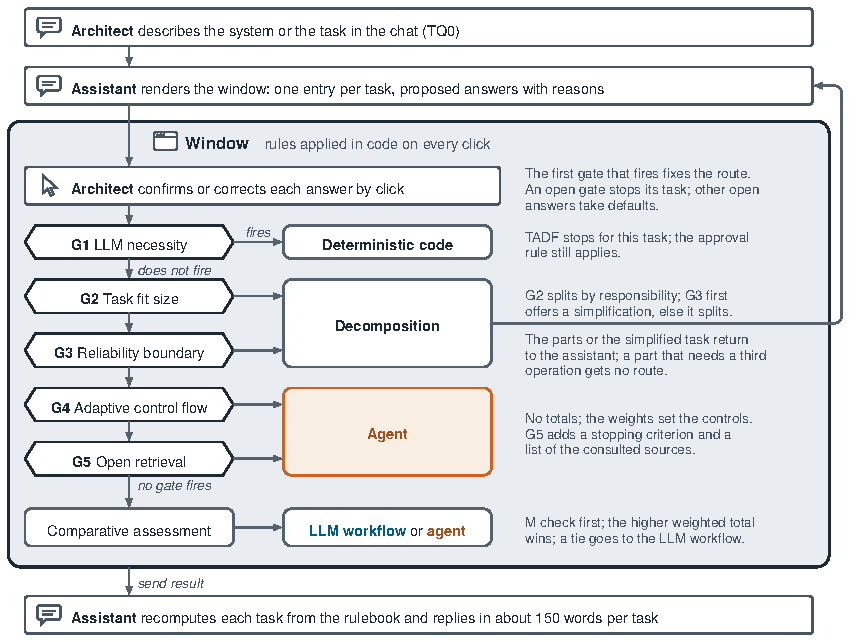
\includegraphics[width=.94\linewidth]{Figures/fig_tadf_final_flow_v2.pdf}
\caption[Routing logic of a TADF consultation in the window]{Routing logic of a TADF consultation in the window, condensed from \texttt{SKILL.md} of the skill \texttt{tadf-final}.}
\label{fig:tadf-flow}
\end{figure}

\subsubsection{Final Capability Matrix and Calculation}
\label{app:artifact/scoring}

Table~\ref{tab:v3-matrix} shows the active matrix. T1 carries weight 3 if its condition is confirmed and 0 otherwise. The architect weights P1--P6 from 0 to 3 and can mark P1, P2, P3 or P5 as mandatory (M). M is accepted only if no later control fully absorbs a violation; otherwise weight 3 applies. The skill calls P1--P6 task-performance indicators, while the thesis calls them deployment indicators.

\begingroup\renewcommand{\baselinestretch}{1}\small\setlength{\tabcolsep}{3pt}\renewcommand{\arraystretch}{1.08}
\begin{longtable}{>{\raggedright\arraybackslash}p{\dimexpr0.070\linewidth-2\tabcolsep\relax} >{\raggedright\arraybackslash}p{\dimexpr0.370\linewidth-2\tabcolsep\relax} >{\raggedright\arraybackslash}p{\dimexpr0.220\linewidth-2\tabcolsep\relax} >{\raggedright\arraybackslash}p{\dimexpr0.100\linewidth-2\tabcolsep\relax} >{\raggedright\arraybackslash}p{\dimexpr0.120\linewidth-2\tabcolsep\relax} >{\raggedright\arraybackslash}p{\dimexpr0.120\linewidth-2\tabcolsep\relax}}
\caption[Capability matrix of the final TADF]{Capability matrix of the final TADF. W: LLM workflow; A: agent.}\label{tab:v3-matrix}\\
\toprule
\textbf{ID} & \textbf{Criterion or deployment indicator} & \textbf{Weight} & \textbf{M allowed} & \textbf{W} & \textbf{A} \\
\midrule
\endfirsthead
\multicolumn{6}{l}{\tablename~\thetable{} (continued)}\\
\toprule
\textbf{ID} & \textbf{Criterion or deployment indicator} & \textbf{Weight} & \textbf{M allowed} & \textbf{W} & \textbf{A} \\
\midrule
\endhead
\bottomrule
\endlastfoot
T1 & Rule application success & 3 if applicable & -- & 3 & 2 \\
\addlinespace
P1 & Traceability & 0--3 or M & yes & 3 & 2 \\
\addlinespace
P2 & Safe failure & 0--3 or M & yes & 3 & 1 \\
\addlinespace
P3 & Schema guarantee & 0--3 or M & yes & 3 & 2 \\
\addlinespace
P4 & Efficiency & 0--3 & no & 3 & 2 \\
\addlinespace
P5 & Robustness to messy input & 0--3 or M & yes & 2 & 3 \\
\addlinespace
P6 & Evolvability & 0--3 & no & 1 & 3 \\
\end{longtable}
\endgroup

For each eligible orchestration paradigm \(p\), the comparative score is
\[
S(p)=\sum_{i\in A}w_i c_{i,p},
\]
where \(A\) contains T1 if it applies and all deployment indicators. M counts as weight 3 but is checked first: capability 1 excludes the orchestration paradigm, and capability 2 makes a control mandatory. The higher total wins, and a tie selects the LLM workflow. A margin of one or two points is checked again and, if it holds, reported as a close call. After the route is fixed, the component rule turns a weight of 2 or more into a mandatory control at capability 2 and into a residual risk that needs a resolution at capability 1. After G4 or G5, M with agent capability 1 is a deployment conflict.

The scores rest on different bases: completion bands at 90 and 50 percent for T1 and P5, construction rubrics for P1 and P3, the observed failure direction for P2, token ratios at 1.5 and 3 times the lower value for P4, and a derivation for P6. They are therefore no common probability scale. At the default weight of 2, the LLM workflow leads by four points and no task-fit criterion favors the agent, so a neutral profile cannot yield an agent recommendation on the comparative path.

\subsubsection{Design Provenance and Evidence Boundaries}
\label{app:artifact/provenance}

Table~\ref{tab:provenance} separates the basis of each design element from the limits of its evidence.

\begingroup
\renewcommand{\baselinestretch}{1}\small
\setlength{\tabcolsep}{3pt}\renewcommand{\arraystretch}{1.08}
\begin{longtable}{>{\raggedright\arraybackslash}p{\dimexpr.24\linewidth-2\tabcolsep\relax} >{\raggedright\arraybackslash}p{\dimexpr.38\linewidth-2\tabcolsep\relax} >{\raggedright\arraybackslash}p{\dimexpr.38\linewidth-2\tabcolsep\relax}}
\caption[Provenance and evidence boundaries of the final TADF]{Provenance and evidence boundaries of the final TADF.}\label{tab:provenance}\\
\toprule
\textbf{Design element} & \textbf{Basis} & \textbf{Evidence boundary}\\
\midrule
\endfirsthead
\multicolumn{3}{l}{\tablename~\thetable{} (continued)}\\
\toprule
\textbf{Design element} & \textbf{Basis} & \textbf{Evidence boundary}\\
\midrule
\endhead
\bottomrule
\endlastfoot
Task as the unit of decision; distinction between the orchestration paradigms & Theoretical background, task taxonomy and the operational definitions of the experiments (Sections~\ref{subsec:theory/workflows-agents}, \ref{subsubsec:TADF/taxonomy}) & A defined scope, not complete coverage of automation architectures. \\
\addlinespace
Gates, T1 and capability scores & Main experimental comparison, deep-dive runs, score rubrics and the initial framework (Sections~\ref{subsubsec:TADF/results}, \ref{subsec:TADF/initial-artifact}) & The gates generalize from selected conditions. P1 and P3 rest on construction, and P6 is derived. The third G3 condition has no measured basis and is kept as a precaution (IT-086). \\
\addlinespace
Skill delivery, system context, definitions and design knowledge & Practitioner interviews and redesign (Section~\ref{subsubsec:TADF/episode1}) & Formative requirements; no comparative usability test and no new capability measurement. \\
\addlinespace
Second G4 question, mandatory minimum and implementation commitment & WorkBench failure diagnosis and executor revision (Section~\ref{subsubsec:TADF/episode2}) & One combined revision without tests of single rules. The measured executor checked conditions and item counts only through prompts, and the new G4 question was not tested again. \\
\addlinespace
Gate block, order of P1--P6, probe for mandatory markings, output structure and fixed-score rule & Pilot consultations and the walkthrough of 27 August 2026 (IT-079 to IT-081; Appendix~\ref{app:artifact/versions}) & Scripted use; independent use and consultation effort were not measured. \\
\addlinespace
Retirement of T3 and T2 & Final structured-retrieval results (49/75 versus 58/75, both band 2) and a confirmation test that gave all nine records the same value (Section~\ref{subsubsec:TADF/evolution}) & Retrieval over known sources and per-item processing remain build knowledge. A new task-fit criterion would need new measurements. \\
\addlinespace
Corrected evidence texts & The defective outcome check of f-med-5 (Appendix~\ref{app:results/contrasts}), the classification of the agent's wrong decisions in D and the records of Episode~2 (IT-084, IT-085) & No score or rule changed. \\
\addlinespace
Consultation window, proposed answers with reasons, rule application in code and short replies & Course and effort of the text consultations of 29 September 2026 (\mbox{IT-087}), the deviations of the walkthrough (\mbox{IT-081}) and the tests of the window against the rulebook (\mbox{IT-088} to \mbox{IT-090}) & Needs a host that can show interactive pages. The effort is compared on two known scenarios with the builder as architect (Section~\ref{subsubsec:TADF/artifact-correction}); independent use was not tested. \\
\end{longtable}
\endgroup

The mandatory minimum combines responses to observed failures with requirements that go beyond the measured executor. The increase from 41.6 to 66.2 percent on WorkBench therefore does not isolate single controls. Likewise, separate calls per criterion in the verification form are a proposed build form: the verification workflow of the main experimental comparison evaluated its five criteria in one structured call before deterministic aggregation (Appendices~\ref{app:protocol/implementation} and~\ref{app:eval2/revision}). A build form, a score threshold or a mandatory component is design knowledge, not verified behavior of a deployed implementation.

\subsubsection{Versions and Iterations}
\label{app:artifact/versions}

Table~\ref{tab:tadf-versions} lists the main states of TADF, their form and how each was assessed. Appendix~\ref{app:evolution/development} details the versions up to v2.2, and Appendix~\ref{app:eval1/improvements} lists the changes after Episode~1. After Episode~2, IT-078 sharpened G4, added the mandatory minimum and the implementation commitment (Section~\ref{subsubsec:TADF/episode2}) and added two build rules: a pilot before an implementation is frozen, and aggregates and superlatives computed in code. It added no gate, threshold, capability score or weight, and it rejected a lifecycle gate, because the lifecycle belongs to the system context. Two simulated pilot consultations on 27 August 2026 then refined the dialogue (IT-079, IT-080). Since then, the deployment indicators are asked in order, explanations are shorter, mandatory markings are task-local and percentages are labelled as comparative fit. Proposed gate answers are confirmed together, and before a mandatory marking is accepted, a probe asks whether a later control absorbs a violation. Replacing selected mandatory markings of safe failure by weight~3 left the recommendations of the pilots unchanged. Their transcripts are not archived. The walkthrough of 27 August 2026 led to the fixed-score rule (IT-081; Appendix~\ref{app:transcripts/audit}). The development log records every iteration with its reason and its change (Appendix~\ref{app:repository/audit}).

\begin{table}[htbp]
\centering
\caption[Versions of TADF, their form and their assessment]{Versions of TADF, their form and their assessment.}
\label{tab:tadf-versions}
\begingroup
\renewcommand{\baselinestretch}{1}\small
\setlength{\tabcolsep}{3pt}
\renewcommand{\arraystretch}{1.08}
\begin{tabular}{>{\raggedright\arraybackslash}p{\dimexpr.22\linewidth-2\tabcolsep\relax} >{\raggedright\arraybackslash}p{\dimexpr.43\linewidth-2\tabcolsep\relax} >{\raggedright\arraybackslash}p{\dimexpr.35\linewidth-2\tabcolsep\relax}}
\toprule
\textbf{Version and date (2026)} & \textbf{Form} & \textbf{Assessment} \\
\midrule
v1 to v2.1, from 15~July & Routing questions in four drafts (list, decision tree, process view and decision table), then gates and weighted scoring in two tables & Deep-dive runs and a structured self-review (Appendix~\ref{app:evolution/development}) \\
\addlinespace
v2.2, frozen on 3~August & Decision Sheet: an Excel workbook that checks five gates for one task and then compares weighted totals & Mechanical checks; Episode~1, practitioner interviews (Section~\ref{subsubsec:TADF/episode1}) \\
\addlinespace
v3, frozen on 25~August & Skill for an LLM assistant: a guided consultation as a text dialogue, plus a headless mode & Episode~2, WorkBench, in benchmark mode (Section~\ref{subsubsec:TADF/episode2}) \\
\addlinespace
v3, revised from 27~August to 29~September & The same skill, revised after Episode~2 and corrected in an evidence audit & Pilot consultations and a walkthrough; text consultation on two scenarios (Appendix~\ref{app:transcripts}) \\
\addlinespace
v3, final state of 1~October & The skill \path{tadf-final}: one consultation window, with a text mode and a headless mode for other uses & Tests of the window code (Appendix~\ref{app:artifact/files}); demonstration (Section~\ref{subsubsec:TADF/artifact-procedure}) \\
\bottomrule
\end{tabular}
\endgroup
\end{table}

\subsection{Demonstration Record and Verification}
\label{app:transcripts}

This appendix documents the text consultations of 29 September 2026 and the window consultations of 1 October 2026, which Sections~\ref{subsubsec:TADF/artifact-correction} and~\ref{subsubsec:TADF/artifact-procedure} summarize. It identifies the transcripts, shows further parts of the text consultations and checks the recorded decisions against the rulebook. The complete dialogues are in the repository (Appendix~\ref{app:repository}).

\subsubsection{Sources}
\label{app:transcripts/source}
\label{app:transcripts/context}

The two text consultations took place on 29 September 2026 in the Claude app with Claude Sonnet~5.5 and the text-interview skill in the state after \mbox{IT-086} (\path{01-framework/tadf/}). The model was confirmed separately, because the export does not record it. The two window consultations followed on 1 October 2026 with the same model and the skill \path{tadf-final/} in the state of \mbox{IT-090}, which the app held as an account plugin with the same files; the memory of the account was off. The Claude data exports contain account data, such as the account identifier, and are therefore not published; the development log records their checksums (IT-087, IT-091). The repository holds Markdown transcripts converted from them in \path{01-framework/demonstration/}, together with the unchanged export of the walkthrough of 27 August 2026 and the checksums of all transcripts. The transcripts keep the visible messages in their original wording and order and omit internal reasoning, file access, tool results and account data. The window transcripts also show the proposed answers of each window as a table and the messages that the window sent to the chat. Messages are numbered from 1 in each transcript, and the figures refer to these numbers. The figures keep the original wording of the messages and mark cuts with [\ldots].

The file-access records of the exports show that the assistant read the procedure, the rulebook and the design knowledge completely in both text consultations, and the document on constructs and scope in the invoice consultation. The text it read matches the files in \path{01-framework/tadf/}, except for the name line at the top of \path{SKILL.md}, which the installation of the skill writes with quotation marks. In the window consultations, every line of the skill files that the assistant read matches the state of \mbox{IT-090}, and both windows equal its template with the window data. Timestamps in the transcripts are Europe/Berlin time. The consultation times in Section~\ref{subsubsec:TADF/artifact-correction} were measured from the timestamps of the exports, without pauses of more than 15 minutes; words count the messages of the assistant without the window code and without the placeholder lines of the export. \path{01-framework/demonstration/consultation-effort/} holds the measured values and the script that measured them.

\subsubsection{Invoice Consultation}
\label{app:transcripts/invoice}

Figure~\ref{fig:demo-invoice-opening} shows how the system context and the task list arose from the first message. Figure~\ref{fig:demo-invoice-record} shows further design knowledge from the verdict and the decision record. The architect confirmed the implementation commitment with the German word ``ja'', and the assistant then wrote the decision record in German. It summarizes the English verdict of message~10.

\begin{figure}[htbp]
\centering
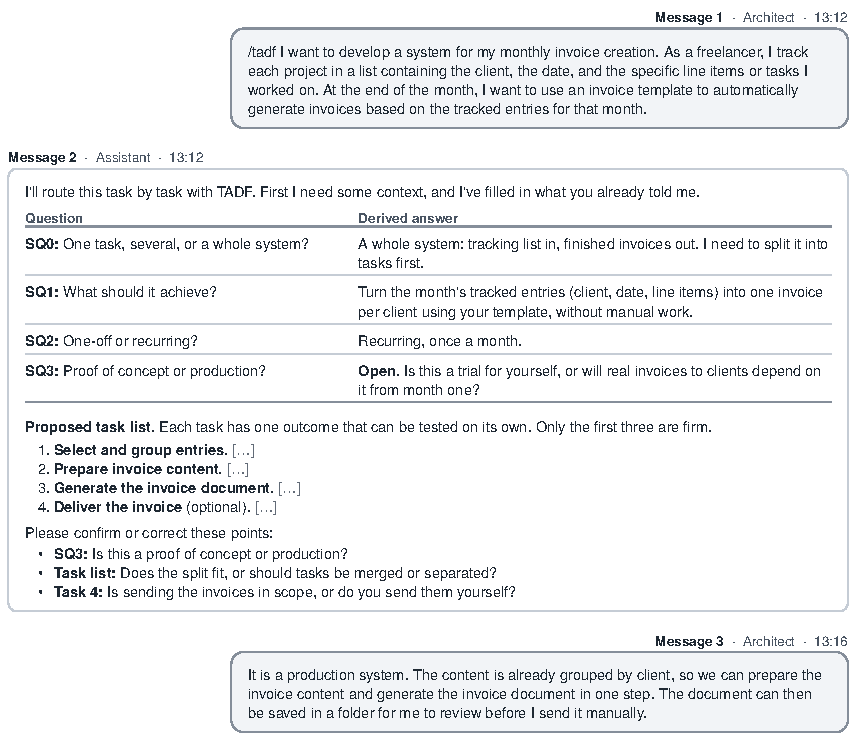
\includegraphics[width=.98\linewidth]{Figures/fig_demo_invoice_opening_v2.pdf}
\caption[Invoice consultation: system context and task list]{Invoice consultation, messages 1--3: system context and task list.}
\label{fig:demo-invoice-opening}
\end{figure}

\begin{figure}[htbp]
\centering
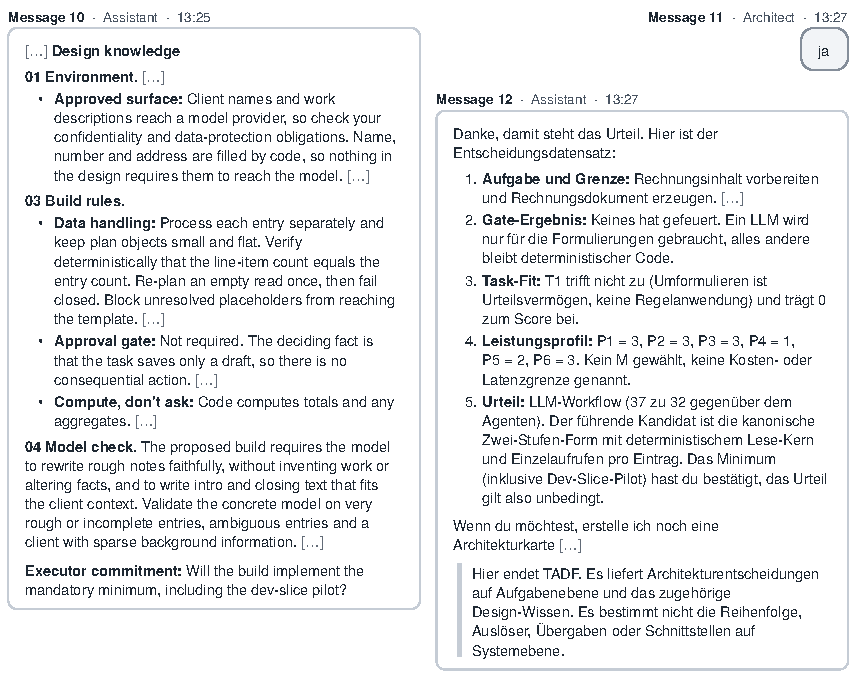
\includegraphics[width=.98\linewidth]{Figures/fig_demo_invoice_record_v2.pdf}
\caption[Invoice consultation: design knowledge and decision record]{Invoice consultation, messages 10--12: design knowledge and decision record.}
\label{fig:demo-invoice-record}
\end{figure}

\subsubsection{CrewAI Consultation}
\label{app:transcripts/crewai}

The scenario was based on \texttt{email\_\allowbreak auto\_\allowbreak responder\_\allowbreak flow}, a publicly available example of CrewAI that checks incoming emails and generates draft responses \parencite{crewaiEmailAutoResponderFlow}. The architect's answers specify the detailed requirements, including human review before sending. They do not describe the behavior of the CrewAI code, which was not evaluated. The same scenario had served in the walkthrough of 27 August 2026.

Figure~\ref{fig:demo-crewai-context} shows the routing of Context gathering. The architect corrected G2 and already named the agent route, but the assistant first clarified G3, because the gates apply in a fixed order. The mandatory marking of safe failure then conflicted with the agent route. The architect resolved the conflict by moving the final readiness decision to deterministic checks outside the loop. The assistant recorded as residual risk what these checks cannot detect, such as a relevant source that was never selected.

For Draft composition, the assistant first counted six simultaneous requirements with a revision round (message~32). The architect answered that code handles exact values, formatting and the output schema and that the model receives one communication profile. The assistant classed this as a simplification that changes the task, the second and last operation on this lineage, and asked which properties the profile fixes and who resolves it (message~34). The architect answered that code resolves the profile from a configuration, which left four requirements, and G3 did not fire (message~36). Figure~\ref{fig:demo-crewai-map} reproduces the architecture map of the closing message.

\begin{figure}[htbp]
\centering
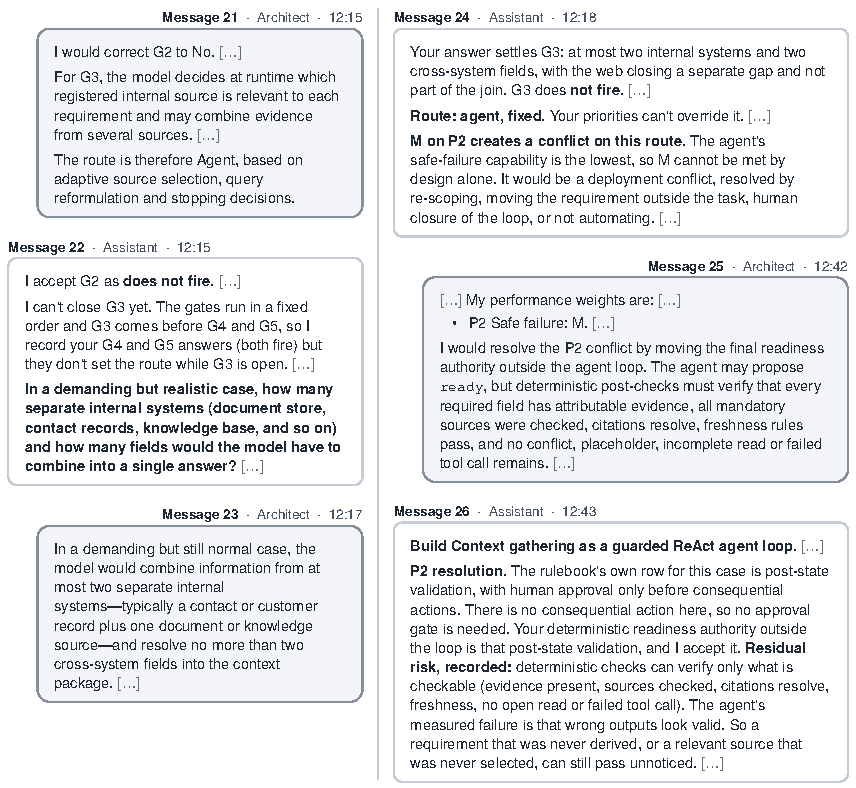
\includegraphics[width=.98\linewidth]{Figures/fig_demo_crewai_context_v2.pdf}
\caption[CrewAI consultation: routing of Context gathering]{CrewAI consultation, messages 21--26: routing of Context gathering.}
\label{fig:demo-crewai-context}
\end{figure}

\begin{figure}[htbp]
\centering
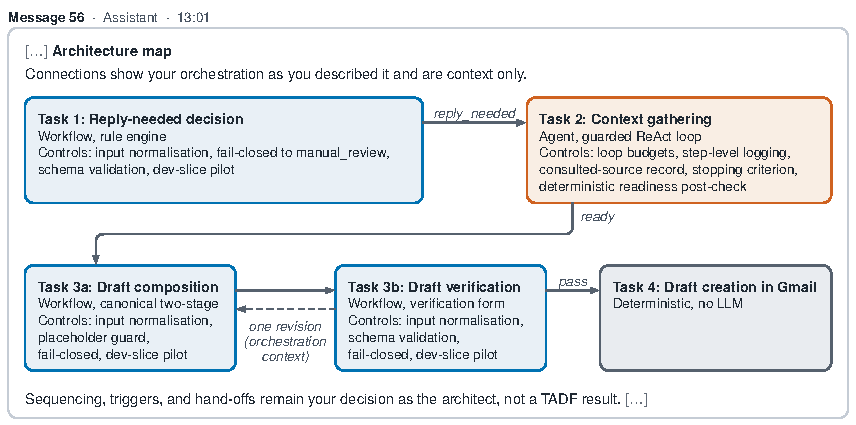
\includegraphics[width=.98\linewidth]{Figures/fig_demo_crewai_map_v2.pdf}
\caption[CrewAI consultation: architecture map]{CrewAI consultation, message 56: architecture map. Node texts, edge labels and connections are those of the Mermaid source; the two-row layout and the colors that mark the three routes were added for the page.}
\label{fig:demo-crewai-map}
\end{figure}

\subsubsection{Decision and Procedure Verification}
\label{app:transcripts/audit}

Table~\ref{tab:demo-audit} checks the recorded decisions against the rulebook. All totals were recomputed from the fixed capability scores and the confirmed weights. The table does not validate the factual answers of the architect.

\begingroup
\renewcommand{\baselinestretch}{1}\small
\setlength{\tabcolsep}{3pt}\renewcommand{\arraystretch}{1.08}
\begin{longtable}{>{\raggedright\arraybackslash}p{\dimexpr.20\linewidth-2\tabcolsep\relax} >{\raggedright\arraybackslash}p{\dimexpr.34\linewidth-2\tabcolsep\relax} >{\raggedright\arraybackslash}p{\dimexpr.46\linewidth-2\tabcolsep\relax}}
\caption[Check of the text consultations against the rulebook]{Check of the text consultations against the rulebook.}\label{tab:demo-audit}\\
\toprule
\textbf{Task and messages} & \textbf{Recorded outcome} & \textbf{Check and limit} \\
\midrule
\endfirsthead
\multicolumn{3}{l}{\tablename~\thetable{} (continued)}\\
\toprule
\textbf{Task and messages} & \textbf{Recorded outcome} & \textbf{Check and limit}\\
\midrule
\endhead
\bottomrule
\endlastfoot
Invoice creation (1--12) & No gate fired; T1 did not apply. P1--P6 weighted 3, 3, 3, 1, 2, 3. LLM workflow, 37 to 32. & Workflow: $9+9+9+3+4+3=37$. Agent: $6+3+6+2+6+9=32$. Input normalization is mandatory (P5), and evolvability is a residual risk (P6). The architect confirmed complete reads with a general answer; the build form still requires reading all pages. \\
\addlinespace
Reply-needed decision (8--17) & No gate fired; T1 applied. P2 and P3 mandatory. LLM workflow with rule engine, 50 points. & $9+9+9+9+6+6+2=50$. P2 as M excludes the agent at capability 1, and the agent columns hold no values. P3 as M alone would have kept the agent eligible. \\
\addlinespace
Context gathering (18--26) & G4 fired, and G5 was recorded. P2 mandatory. Agent, guarded ReAct loop. & The route is fixed, so there is no total. M with agent capability 1 after G4 is a deployment conflict, resolved here by post-state validation. The proposed checks are a design, not a tested control, and cannot show that no relevant source was missed; the verdict records this residual risk. \\
\addlinespace
Draft writing (26--30) & G2 fired. Decomposition into Draft composition and Draft verification. & The parent receives no profile. This is the first operation on the lineage. \\
\addlinespace
Draft composition (30--41) & Simplification, then no gate. P1--P6 weighted 3, 3, 3, 2, 3, 2. LLM workflow, canonical two-stage form, 41 to 34. & Workflow: $9+9+9+6+6+2=41$. Agent: $6+3+6+4+9+6=34$. The margin of seven points is not a close call. The simplification was the second and last operation on the lineage. \\
\addlinespace
Draft verification (42--51) & No gate fired; T1 did not apply. P2 and P3 mandatory. LLM workflow, verification form, 41 points. & $9+9+9+6+6+2=41$. P2 as M excludes the agent. Verification parity in cost was named as context, and the score stayed fixed. That three model-judged criteria lie within the measured five-criterion rubric does not validate this rubric. \\
\addlinespace
Draft creation in Gmail (52--56) & G1 fired. Deterministic implementation. & No profile and no design knowledge, as the rulebook prescribes. \\
\end{longtable}
\endgroup

The walkthrough of 27 August 2026 (IT-081) used the same scenario with the state before the fixed-score rule, when T3 and T2 were still scored. Its record showed five deviations: a stated total of 41 whose contributions summed to 50, agent contributions changed through the efficiency exception, values in the columns of an excluded agent, no implementation commitment and no separate G4 question on complete reads. None of them recurred in the repeated consultation. The four verdicts for an LLM workflow cite 41.6 and 66.2 percent success without and with the mandatory minimum. They need the qualification of Appendix~\ref{app:artifact/provenance}: the measured executor implemented parts of the minimum only through prompts. \mbox{IT-089} reduced these sentences in the skill to what the records show.

\subsubsection{Window Consultations}
\label{app:transcripts/window}

The window consultations of 1 October 2026 used the same two scenarios (\mbox{IT-091}). In each, the assistant showed one window with proposed answers, the architect answered by click and sent the result, and the assistant replied once. The windows proposed 19 and 45 answers. The architect kept 18 and 40 of them, changed 1 and 5 and answered 1 and 18 further questions without a proposal. The architect answered several questions differently from the text consultations. In invoice creation, traceability was weighted 2 and evolvability 1. In the email scenario, the reply-needed decision had no task-fit criterion and no mandatory marking, and draft writing was not split, so its two parts were not routed. Table~\ref{tab:demo-window-audit} checks the recorded decisions against the rulebook. In both consultations, the assistant's recomputation agreed with the window, and no capability score was changed. The assistant pointed out four answers that seemed inconsistent with the description and said whether a change would alter the route, but it left the answers to the architect.

\begingroup
\renewcommand{\baselinestretch}{1}\small
\setlength{\tabcolsep}{3pt}\renewcommand{\arraystretch}{1.08}
\begin{longtable}{>{\raggedright\arraybackslash}p{\dimexpr.20\linewidth-2\tabcolsep\relax} >{\raggedright\arraybackslash}p{\dimexpr.34\linewidth-2\tabcolsep\relax} >{\raggedright\arraybackslash}p{\dimexpr.46\linewidth-2\tabcolsep\relax}}
\caption[Check of the window consultations against the rulebook]{Check of the window consultations against the rulebook.}\label{tab:demo-window-audit}\\
\toprule
\textbf{Task} & \textbf{Recorded outcome} & \textbf{Check and note} \\
\midrule
\endfirsthead
\multicolumn{3}{l}{\tablename~\thetable{} (continued)}\\
\toprule
\textbf{Task} & \textbf{Recorded outcome} & \textbf{Check and note}\\
\midrule
\endhead
\bottomrule
\endlastfoot
Invoice creation & No gate fired; T1 did not apply. P1--P6 weighted 2, 3, 3, 1, 2, 1. LLM workflow, 32 to 24. & Workflow: $6+9+9+3+4+1=32$. Agent: $4+3+6+2+6+3=24$. Input normalization is mandatory (P5), and evolvability is an accepted limitation (P6). The assistant noted that its proposed weight of 3 for P5 would give 34 to 27. \\
\addlinespace
Reply-needed decision & No gate fired; T1 did not apply. P1--P6 weighted 2, 3, 3, 2, 2, 1. LLM workflow, 35 to 26. & Workflow: $6+9+9+6+4+1=35$. Agent: $4+3+6+4+6+3=26$. The efficiency exception of batch classification was named as context only; the score stayed fixed. The assistant noted its proposed weight of 3 for P5. \\
\addlinespace
Context gathering & G4 fired: the model must replan, and the planned reads cannot show the whole deciding state. Agent, ReAct loop. & The route is fixed, so there is no total. Controls are mandatory for P1, P3 and P4, and P2 at weight 2 is a residual risk. The assistant noted that this weight seemed inconsistent with the fail-closed requirement of the description. \\
\addlinespace
Draft writing & No gate fired, because the architect answered G3a with no instead of the proposed yes. P2 mandatory. LLM workflow, 35; agent excluded. & Workflow: $9+9+9+3+4+1=35$. P2 as M excludes the agent at capability 1. The assistant noted that the seven simultaneous requirements with a revision round described in the task would fire G3. \\
\addlinespace
Draft creation in Gmail & G1 fired. Deterministic implementation. & No profile and no design knowledge, as the rulebook prescribes. \\
\end{longtable}
\endgroup

These records bound the role of the consultations. They show how the instrument elicits requirements, applies its rules and records its decisions. They do not measure the task success, token cost or safety of the recommended builds, and one consultation per scenario does not establish unaided use or reliable application with other models. The window consultations used partly different answers than the text consultations, so they illustrate the effect of the window and do not measure it.